\documentclass[11pt]{beamer} % mathserif for normal math fonts.
\usefonttheme[onlymath]{serif}
\usepackage[utf8]{inputenc}
\usepackage[swedish,english]{babel}
\usepackage{amsmath,mathtools}
\usepackage{calc}
\usepackage{tikz}
\usepackage[T1]{fontenc}
\usepackage{comment}
\usepackage{wallpaper}
\usepackage{graphics}
%\usepackage[dvips]{graphics} 
\usepackage{color}

% The Chalmers theme:
\usetheme[titleflower=true]{chalmers} % titleflower = true or false
\title{Modelling of Digital Radar}
%\subtitle{Nonlinear effects on detectability for radar array} % optional
\author[Albin Jonasson Svärdsby]{} % [short author (optional)]{many authors}
\institute{Chalmers University of Technology}
\titlepageextra{Presentation} % Optional extra info, appears before date on title page
\footer{\insertshortauthor\ Some conference} % optional, manually sets footer (default is short author)
%\footer{Something completely different} % but it can of course be anything.
\titlepagelogofile{figures/Avancez_black} % File name to the file you want to include.
%\titlepagelogo{\tikz{\draw(0,0) circle (1);}} % or draw anything for a logo

%%%%%%%%%%%%%%%%%%%%%%%%%%%%%%%%%%%%%%%%%%
\begin{document}

%\setlength{\footertextwidth}{0.5\paperwidth} % You might need to adjust this if the text doesn't fit well.

\section{Title page} % Sections are shown at the bottom left. There is also links in many pdf-readers
\begin{frame}[plain]
 \titlepage
\end{frame}

\begin{frame}
\frametitle{Setup}
 \begin{figure}[h!]\centering
            \scalebox{0.7}{
                \input{figures/Setup/antennConfigEstetHalfSize.pdf_t}
            }
        \end{figure}
\end{frame}


\begin{frame}
\frametitle{Setup}
 \begin{figure}[h!]\centering
            \scalebox{0.7}{
                \input{figures/Setup/echoCalc.pdf_t}
            }
        \end{figure}
\end{frame}



\section{Another section}
\begin{frame}
 \frametitle{Data handling}
% \framesubtitle{With subtitle}

\begin{figure}
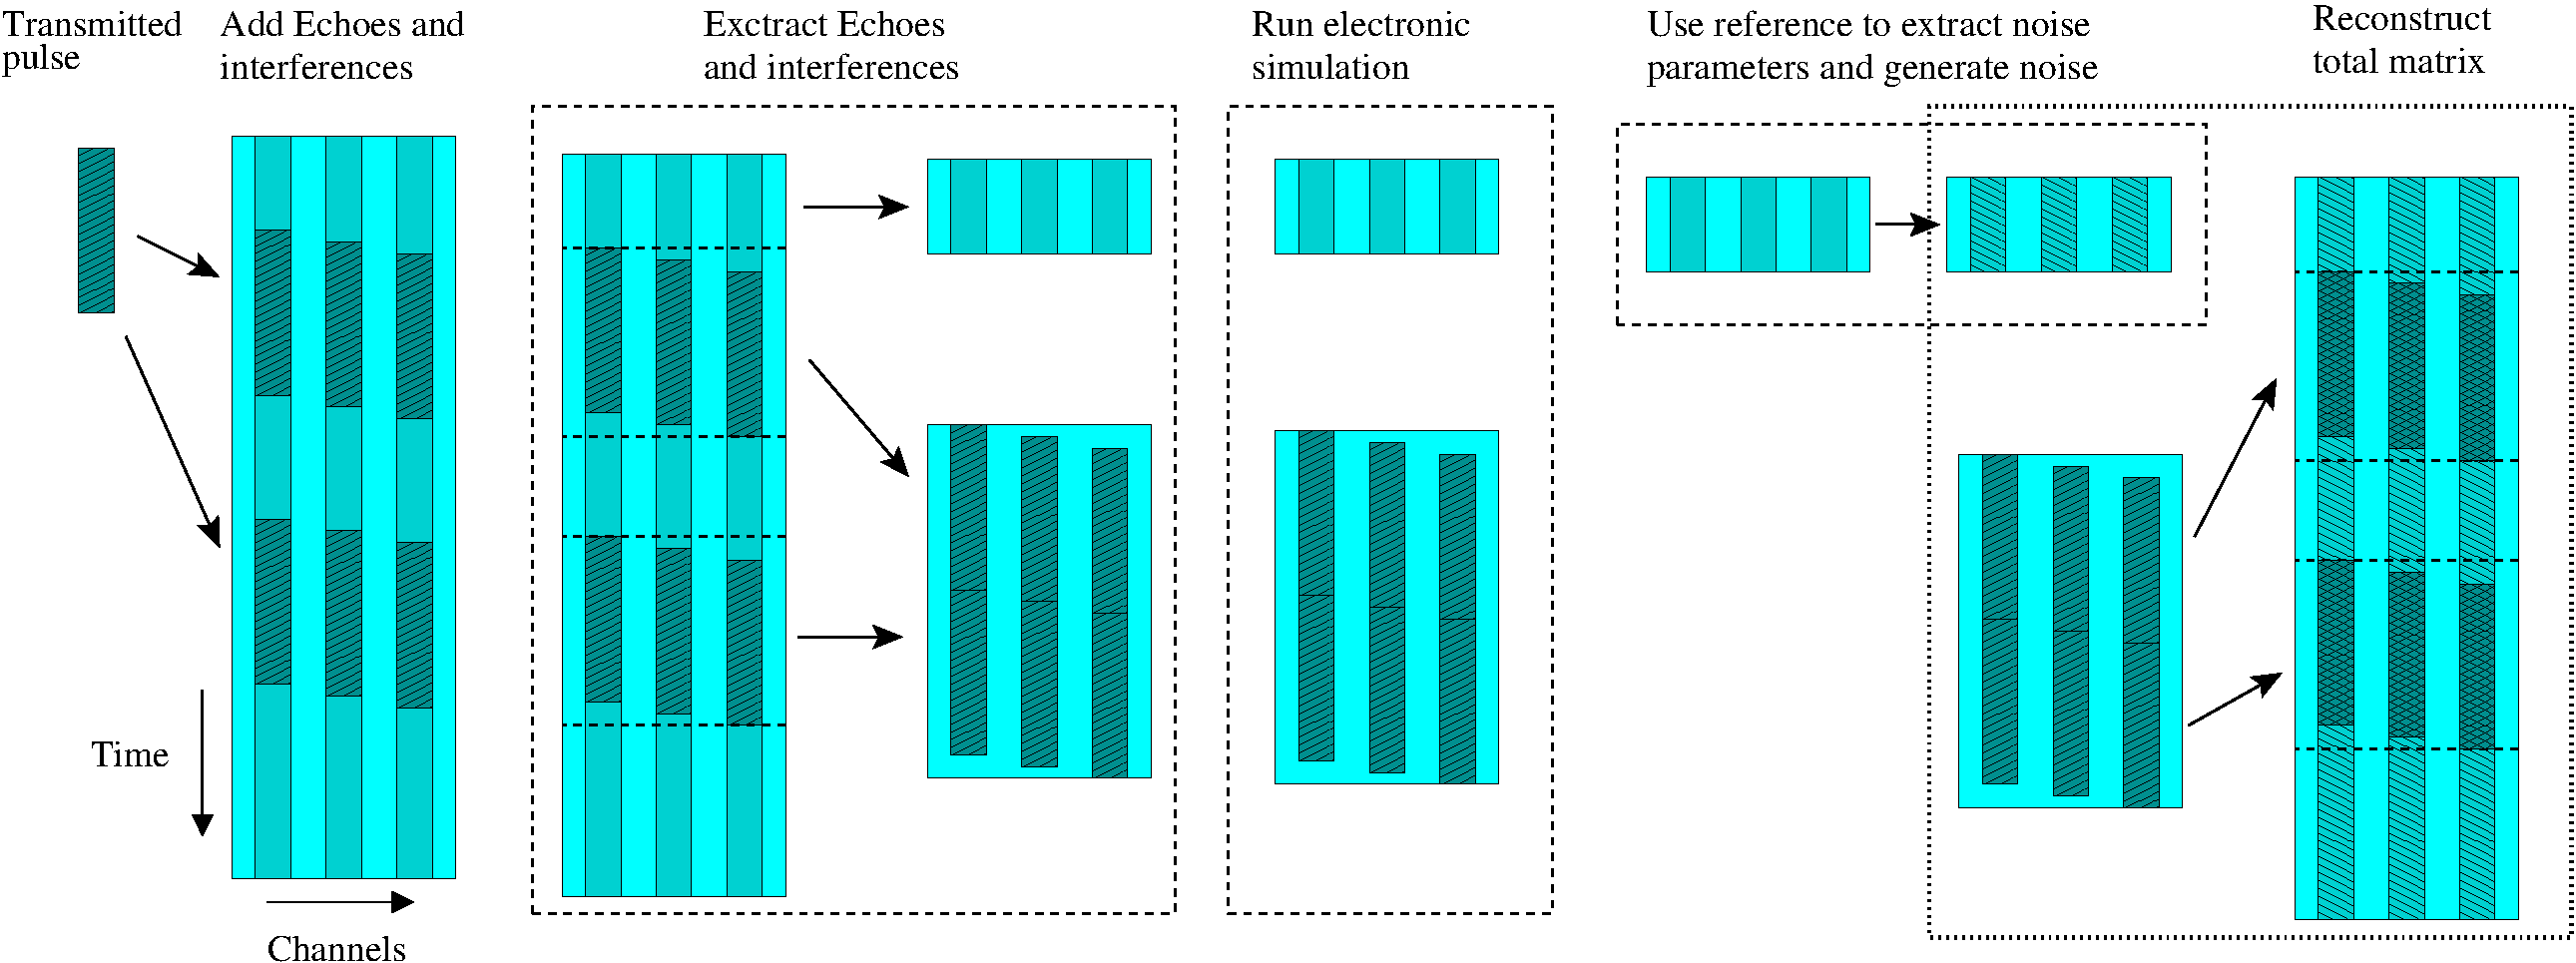
\includegraphics[width=1.05\textwidth]{figures/Setup/channelDataTreatment.pdf}
\end{figure}

\end{frame}



\section{Another section}
\begin{frame}
 \frametitle{Propagation module}
 \framesubtitle{Sequence diagram}

\begin{figure}
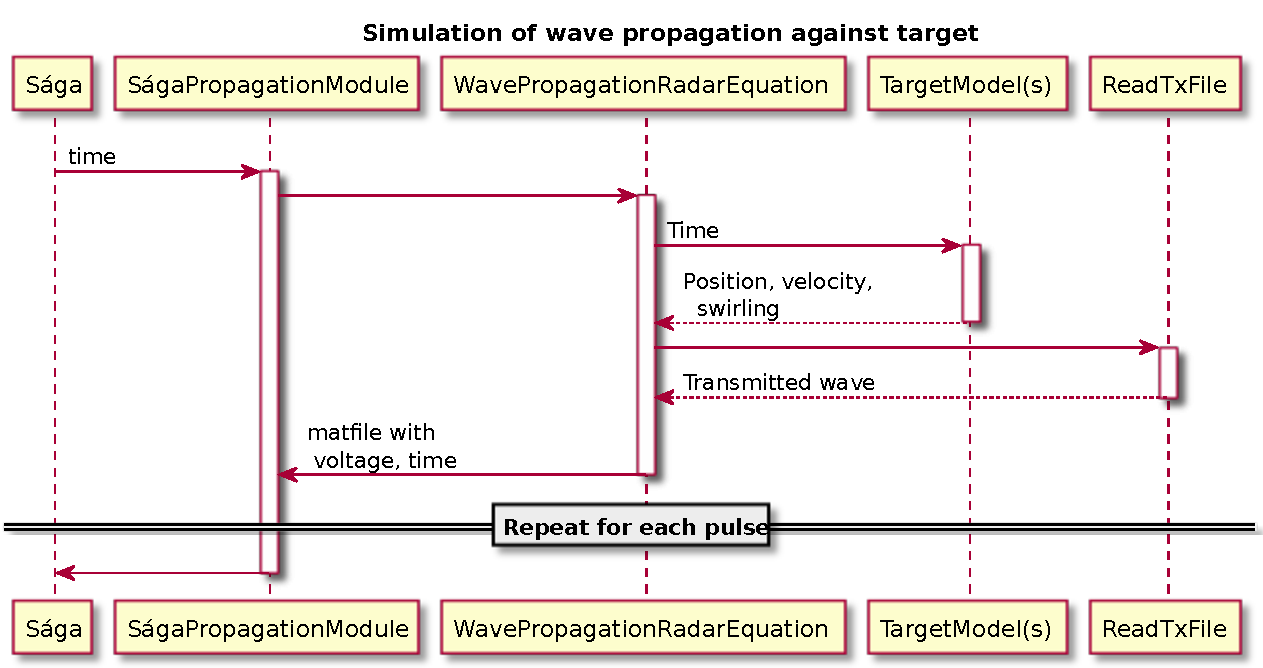
\includegraphics[width=0.9\textwidth]{figures/UML/uml_SagaPropagationModule.pdf}
\end{figure}

\end{frame}


\section{Another section}
\begin{frame}
 \frametitle{Rx module}
 \framesubtitle{Sequence diagram}

\begin{figure}
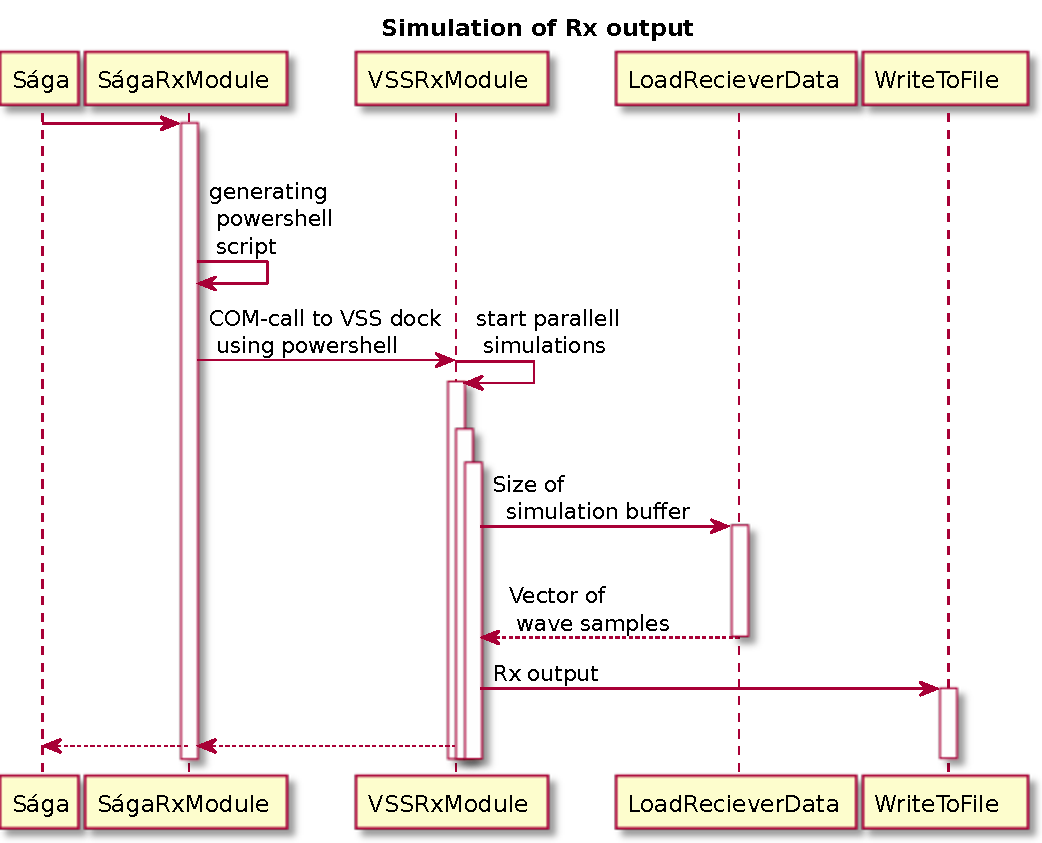
\includegraphics[width=0.75\textwidth]{figures/UML/uml_SagaRx.pdf}
\end{figure}

\end{frame}

\section{Another section}
\begin{frame}
 \frametitle{Tx module}
 \framesubtitle{Sequence diagram}

\begin{figure}
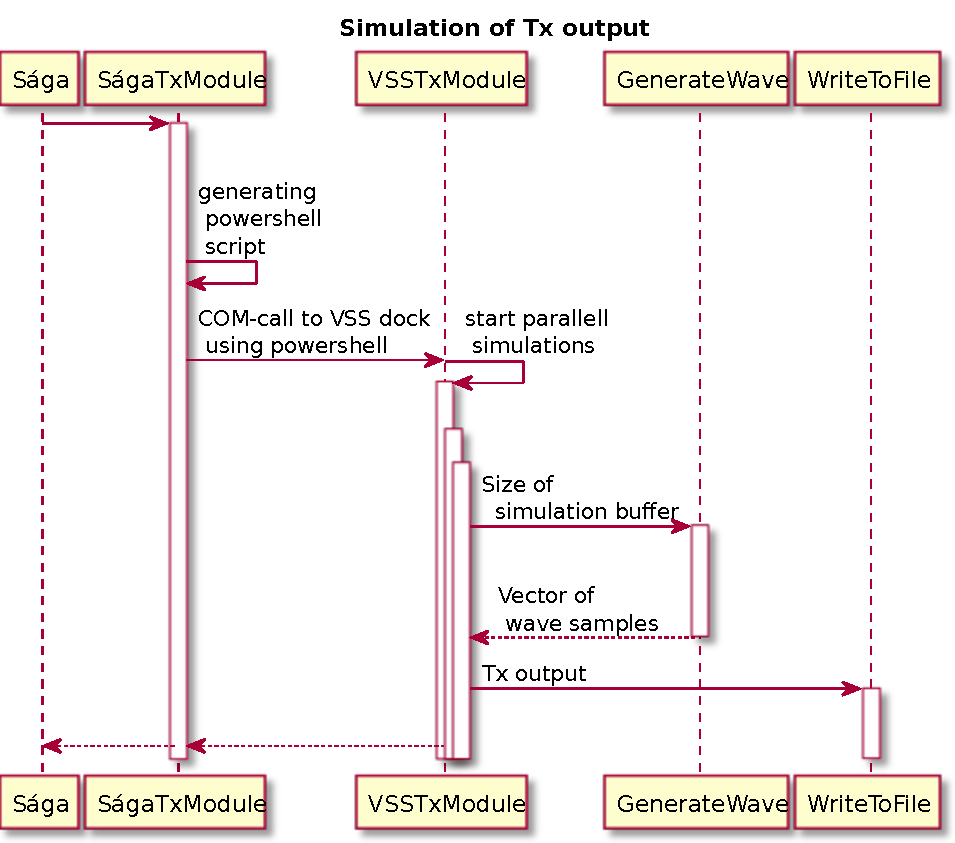
\includegraphics[width=0.75\textwidth]{figures/UML/uml_SagaTx.pdf}
\end{figure}

\end{frame}



\begin{frame}
 \frametitle{Signal after Rx}
 \begin{columns}[T]
        \begin{column}{.5\textwidth}
           
            \begin{figure}
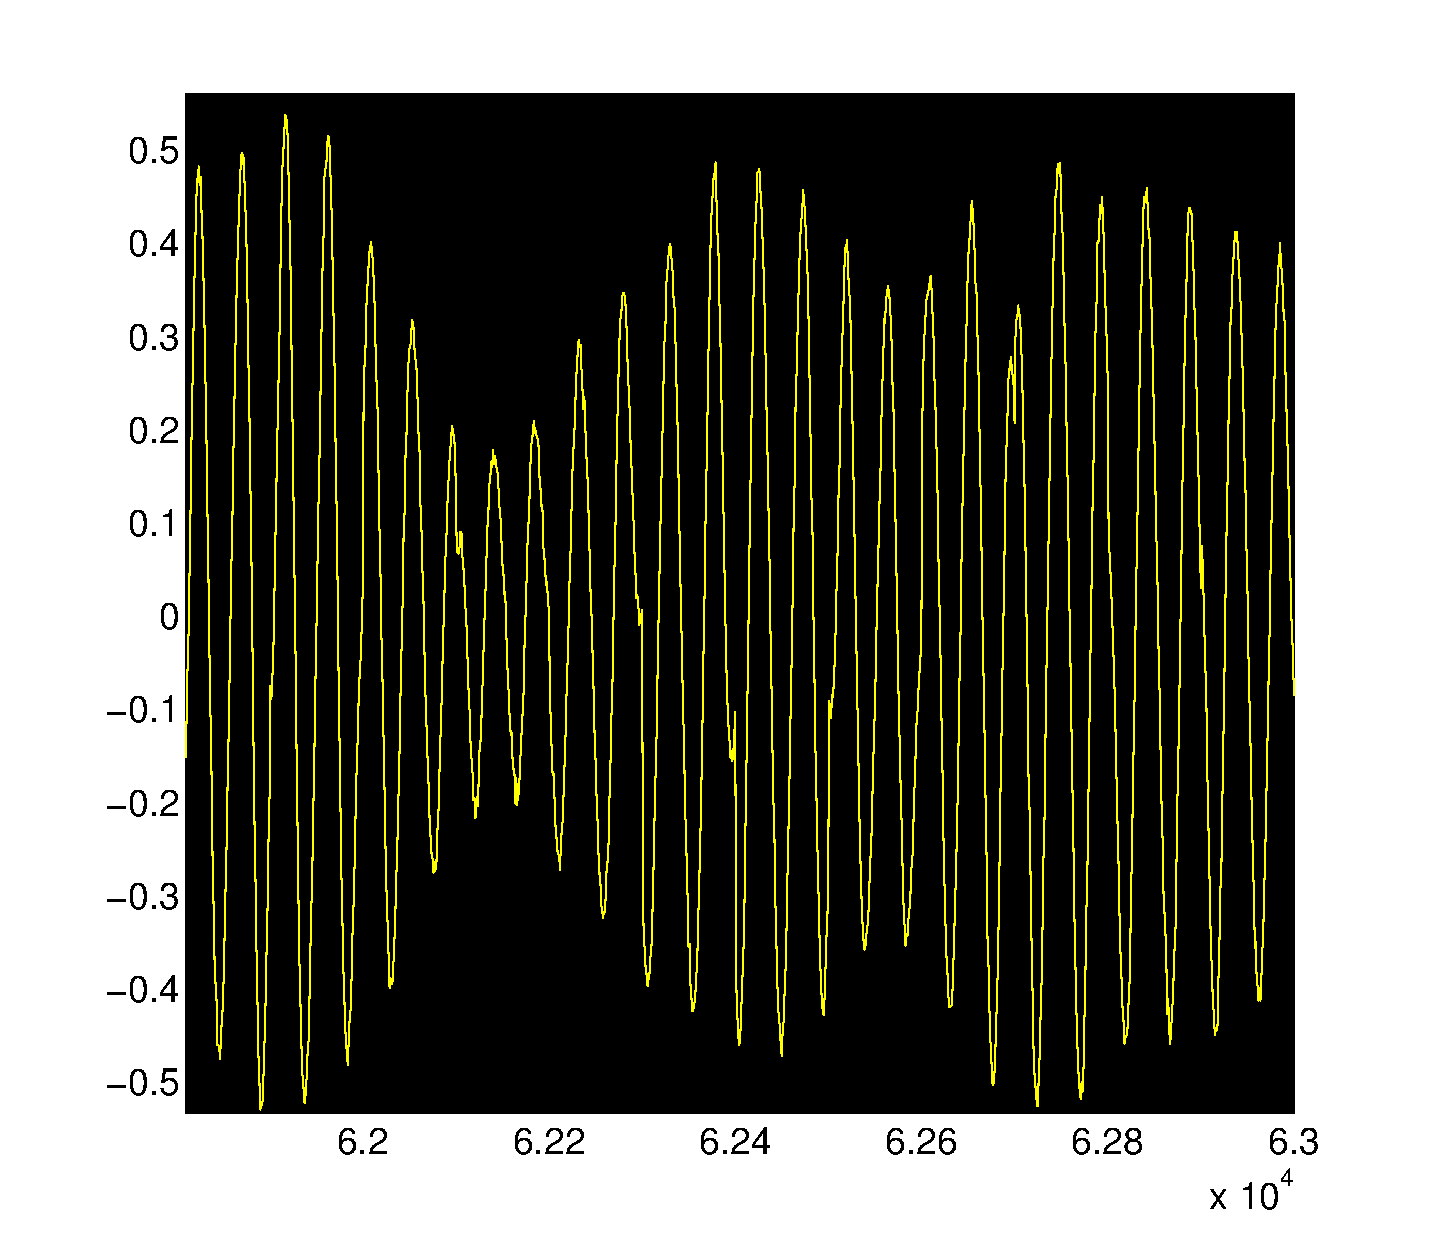
\includegraphics[width=1\textwidth]{Figures/RxEkosignalStarkEjMattnad.pdf}
\end{figure}
 
        \end{column}
         \begin{column}{.5\textwidth}

      \begin{figure}
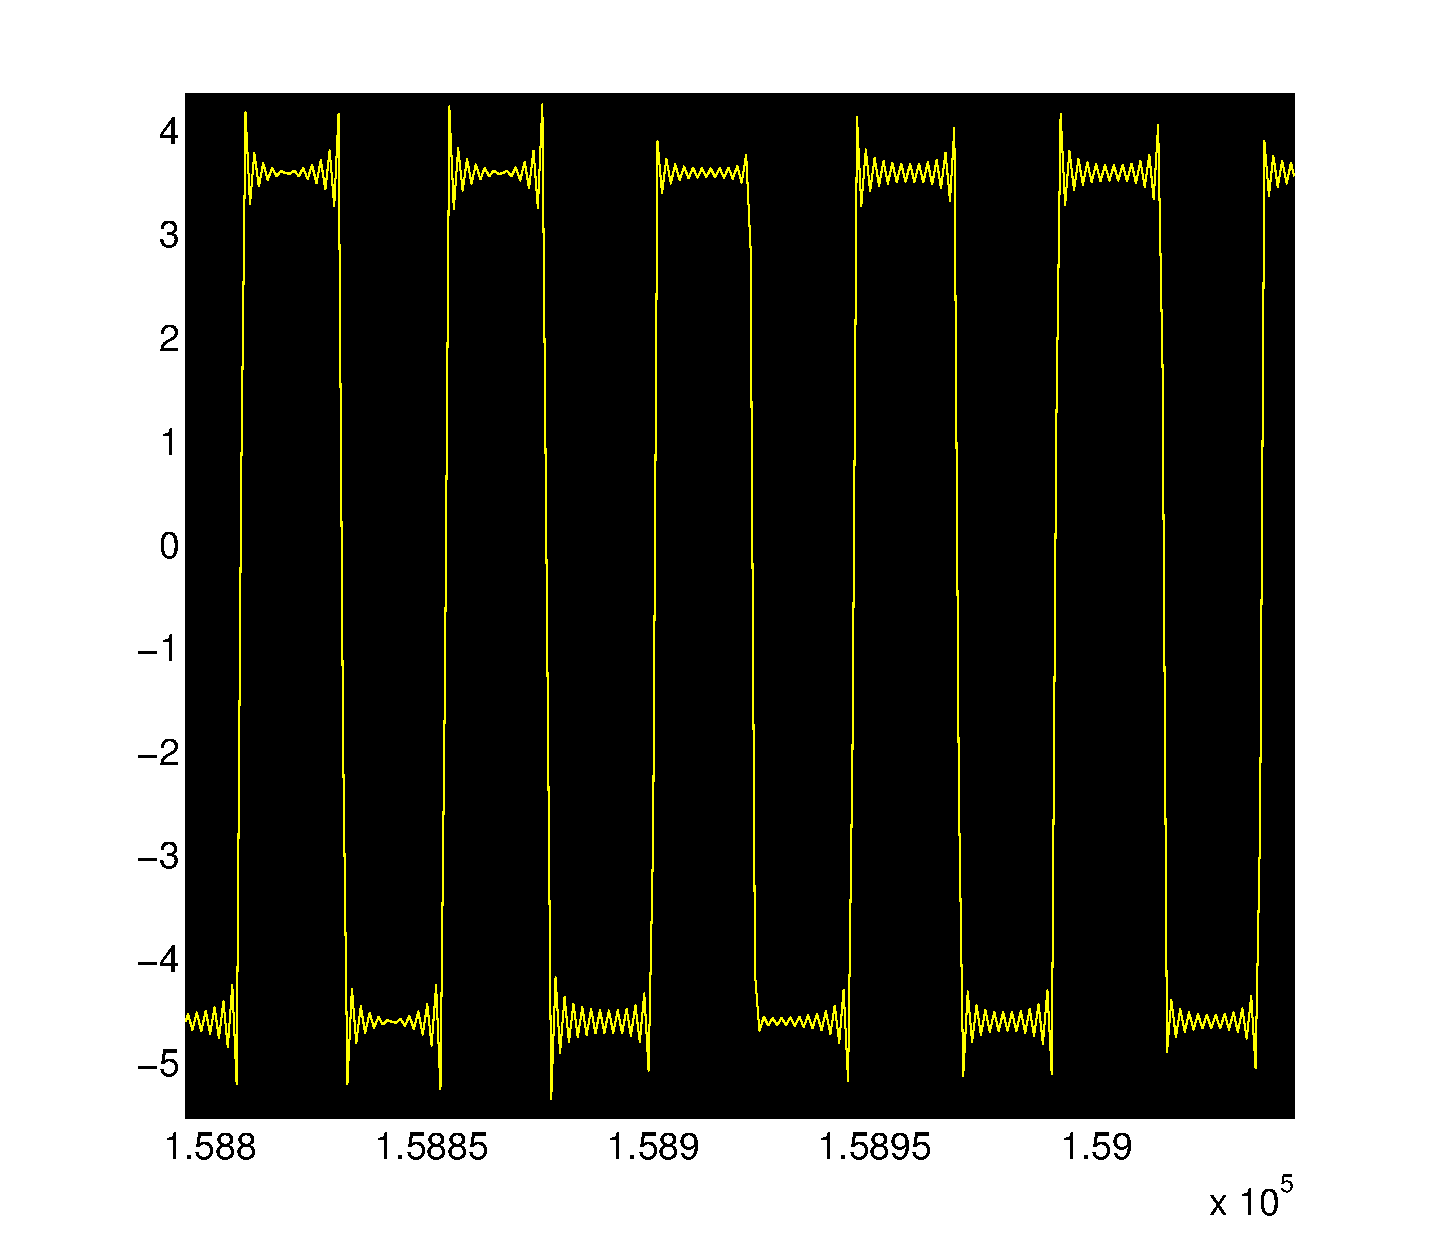
\includegraphics[width=1\textwidth]{Figures/RxEkosignalStarkMattnad.pdf}
\end{figure}

        \end{column}
\end{columns}
\end{frame}





\begin{frame}
 \frametitle{Sampling of signal}
\framesubtitle{Tx}
 \begin{columns}[T]
        \begin{column}{.5\textwidth}
           
       \begin{figure}
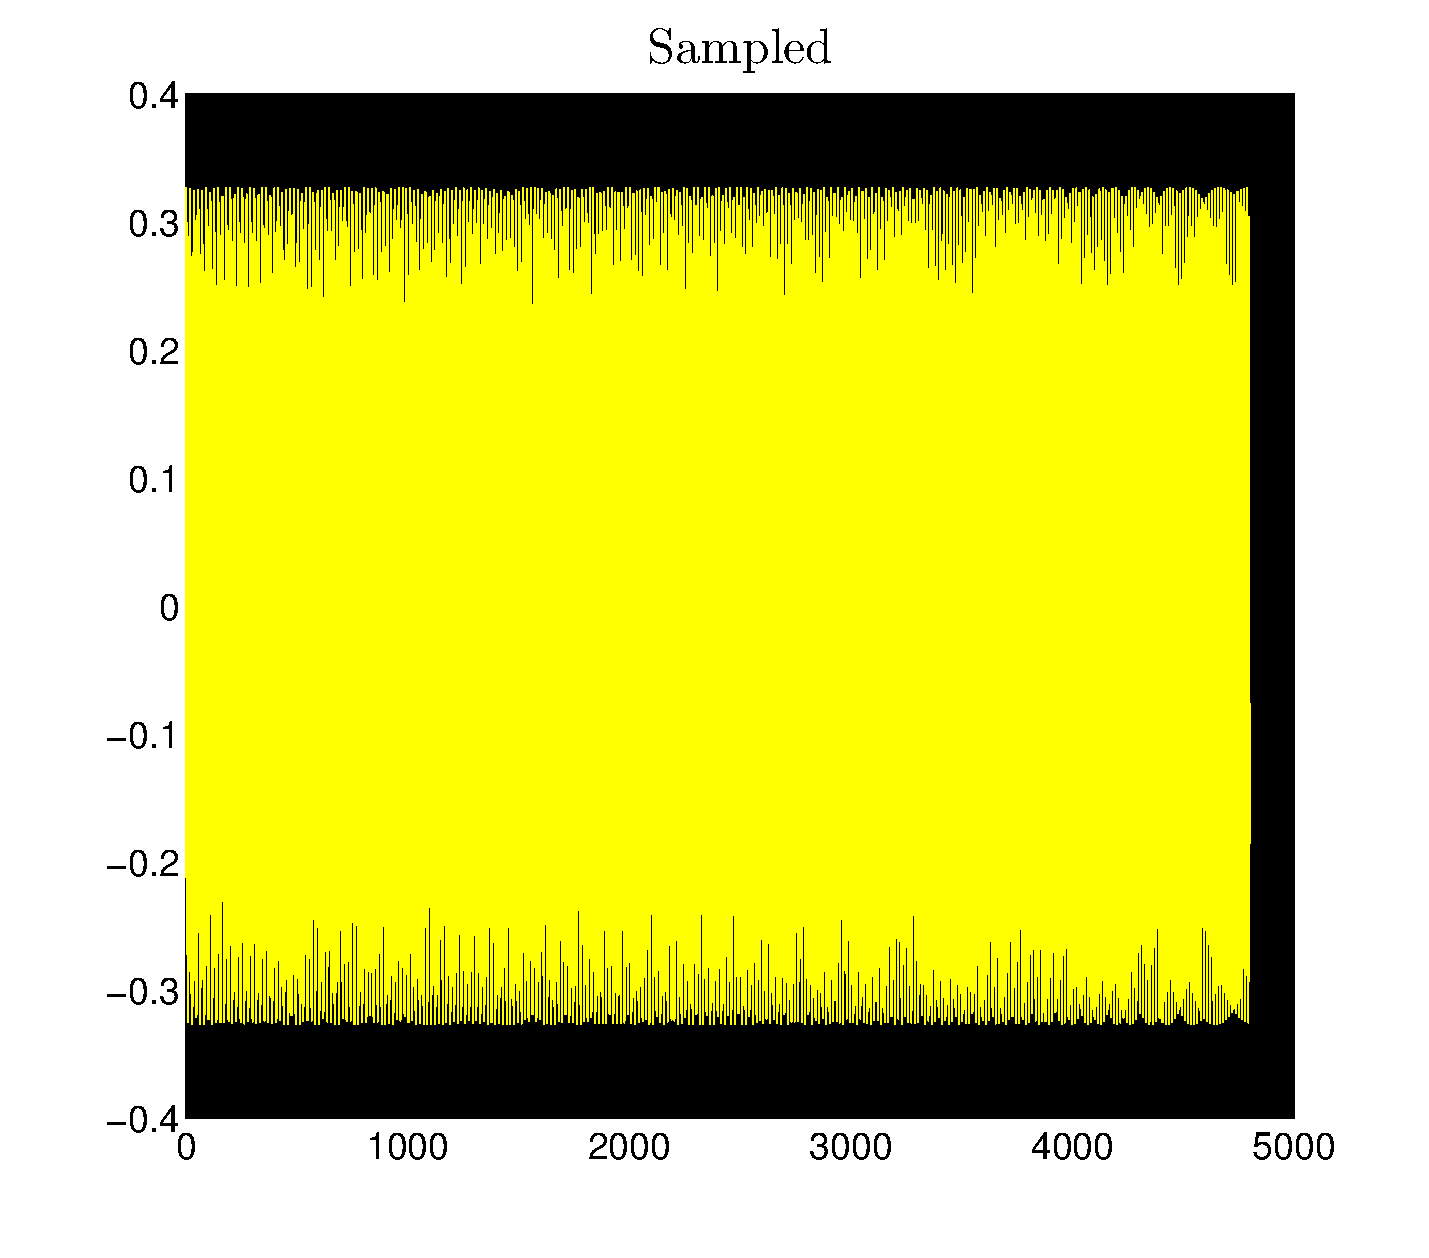
\includegraphics[width=1\textwidth]{Figures/SampledTx.pdf}
\end{figure}
        \end{column}
         \begin{column}{.5\textwidth}

     \begin{figure}
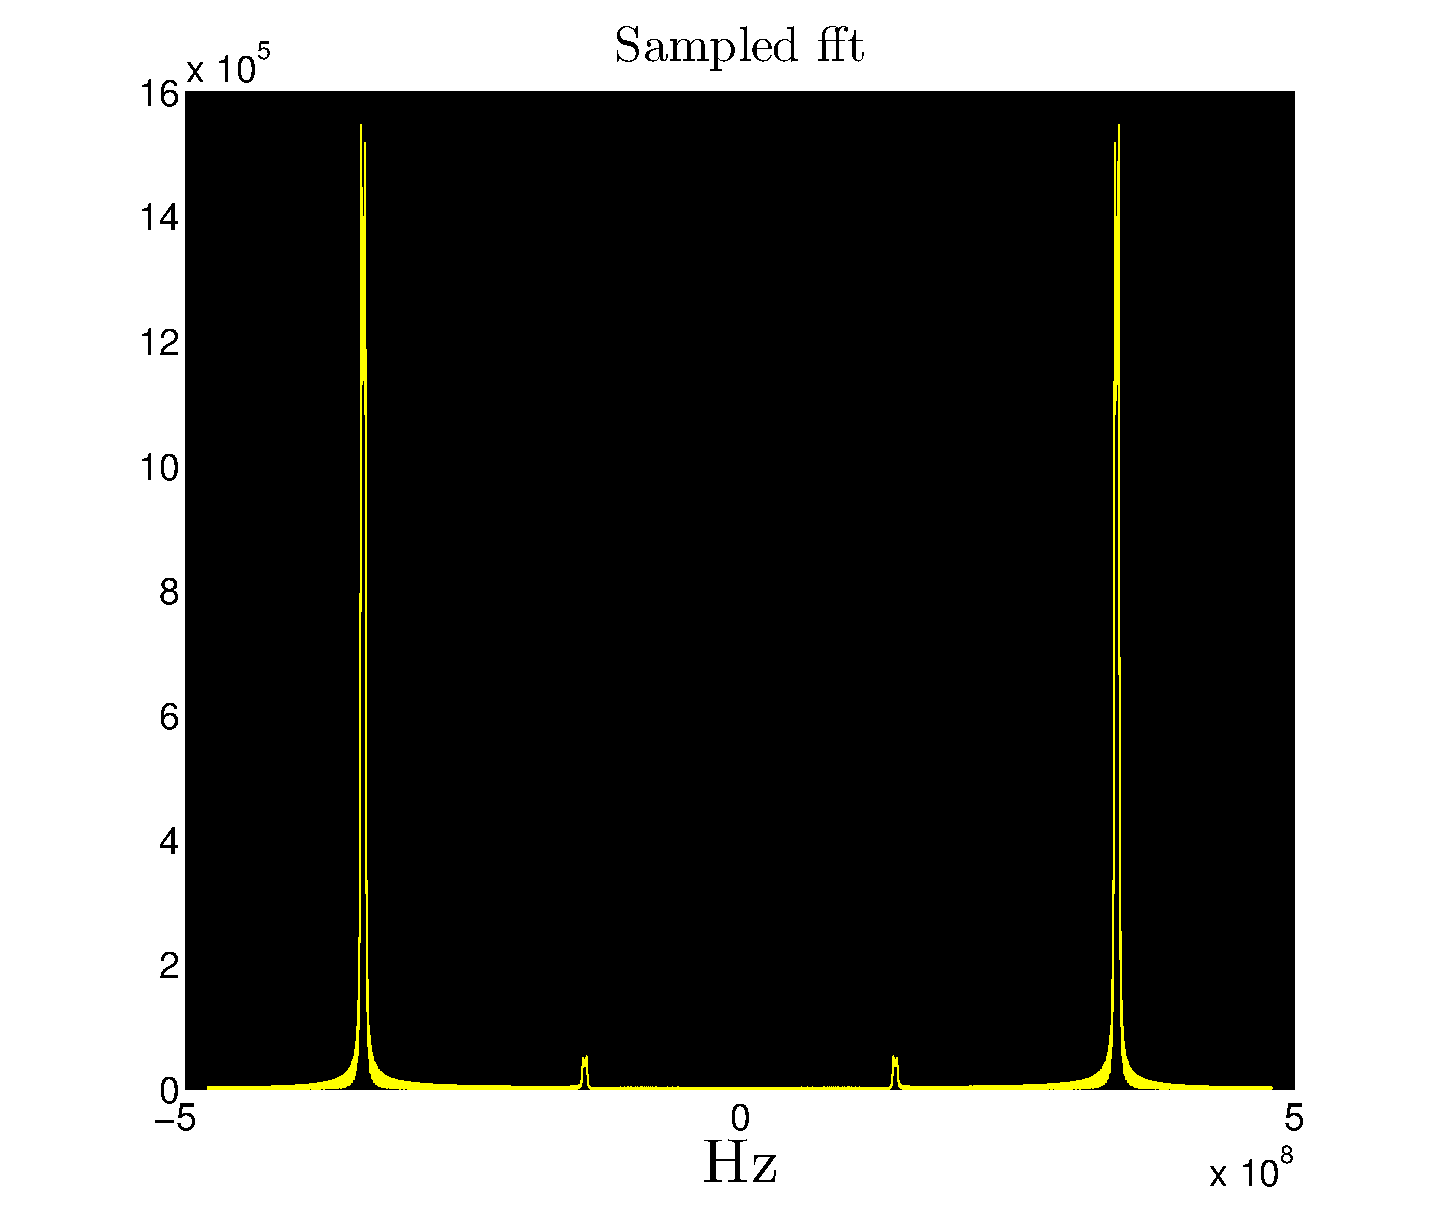
\includegraphics[width=1\textwidth]{Figures/SampledTxFft.pdf}
\end{figure}
        \end{column}
\end{columns}
\end{frame}


\begin{frame}
 \frametitle{convert to baseband}
\framesubtitle{Tx}

 \begin{columns}[T]
        \begin{column}{.5\textwidth}
           
      \begin{figure}
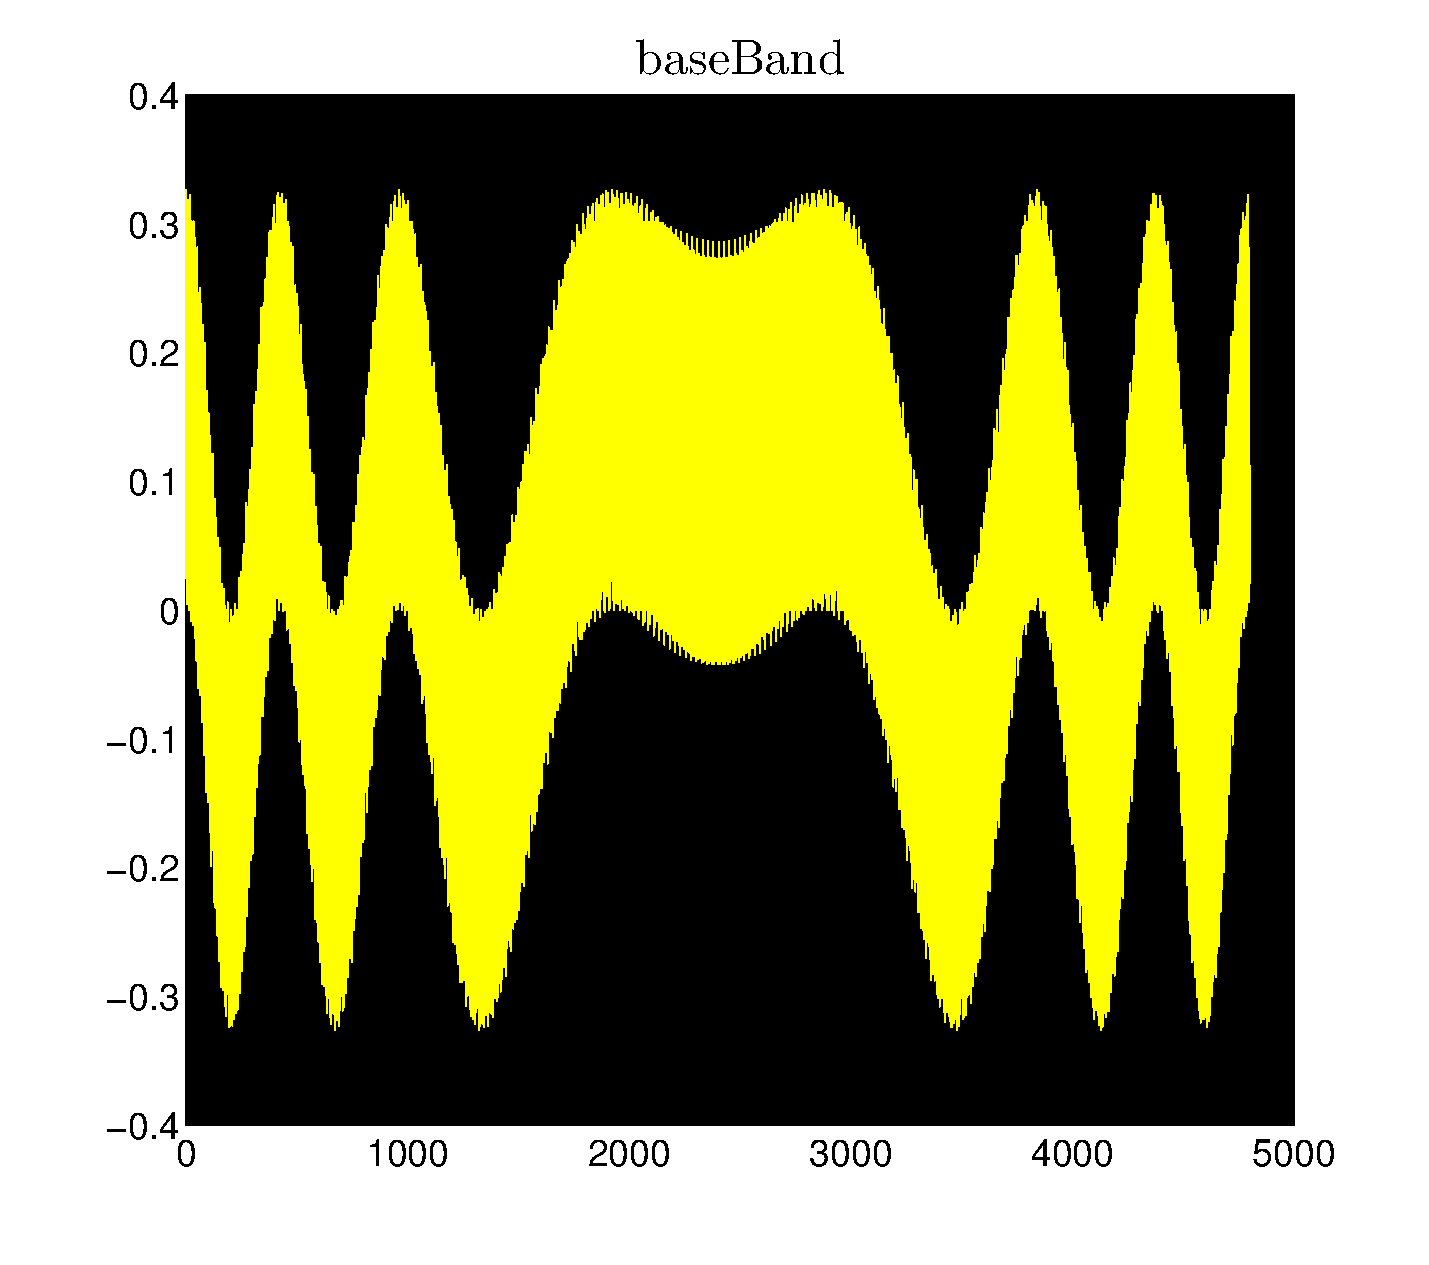
\includegraphics[width=1\textwidth]{Figures/SampledTxBase.pdf}
\end{figure}
        \end{column}
         \begin{column}{.5\textwidth}

    \begin{figure}
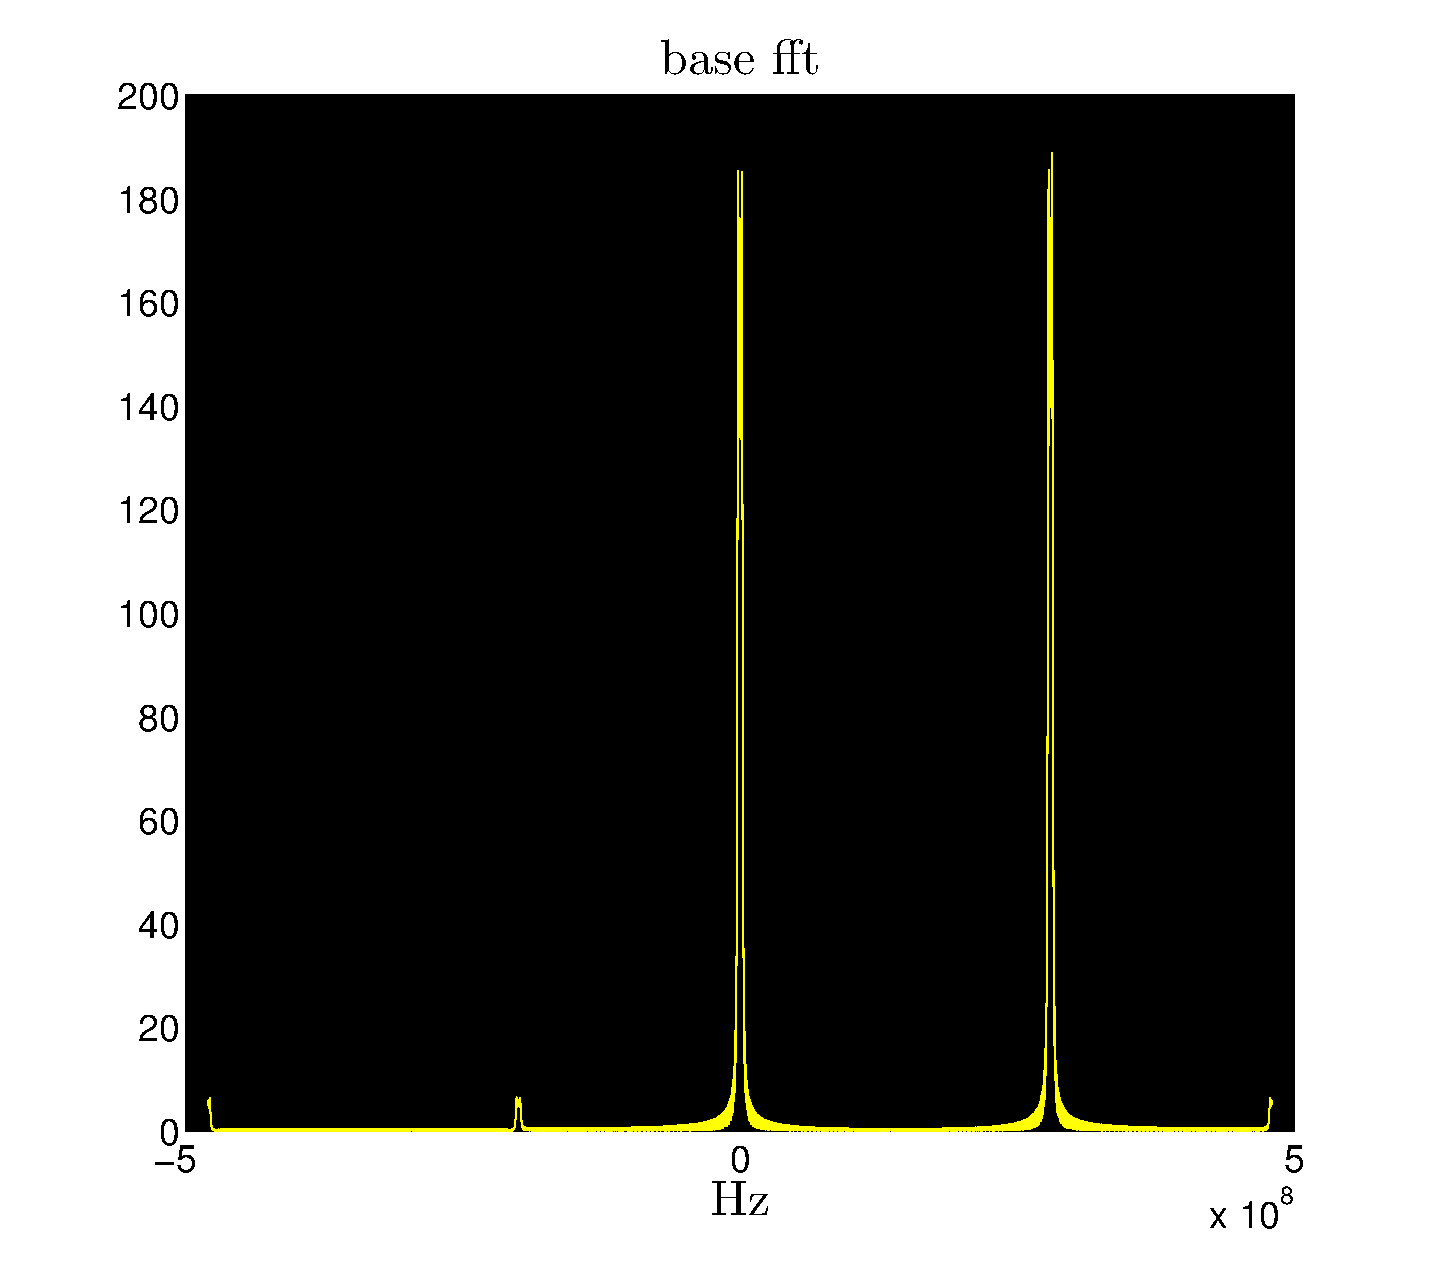
\includegraphics[width=1\textwidth]{Figures/SampledTxBasefft.pdf}
\end{figure}
        \end{column}
\end{columns}
\end{frame}


\begin{frame}
 \frametitle{LP filter and rangebinrate ("Fålltakt")}
 \begin{columns}[T]
        \begin{column}{.5\textwidth}
           
      \begin{figure}
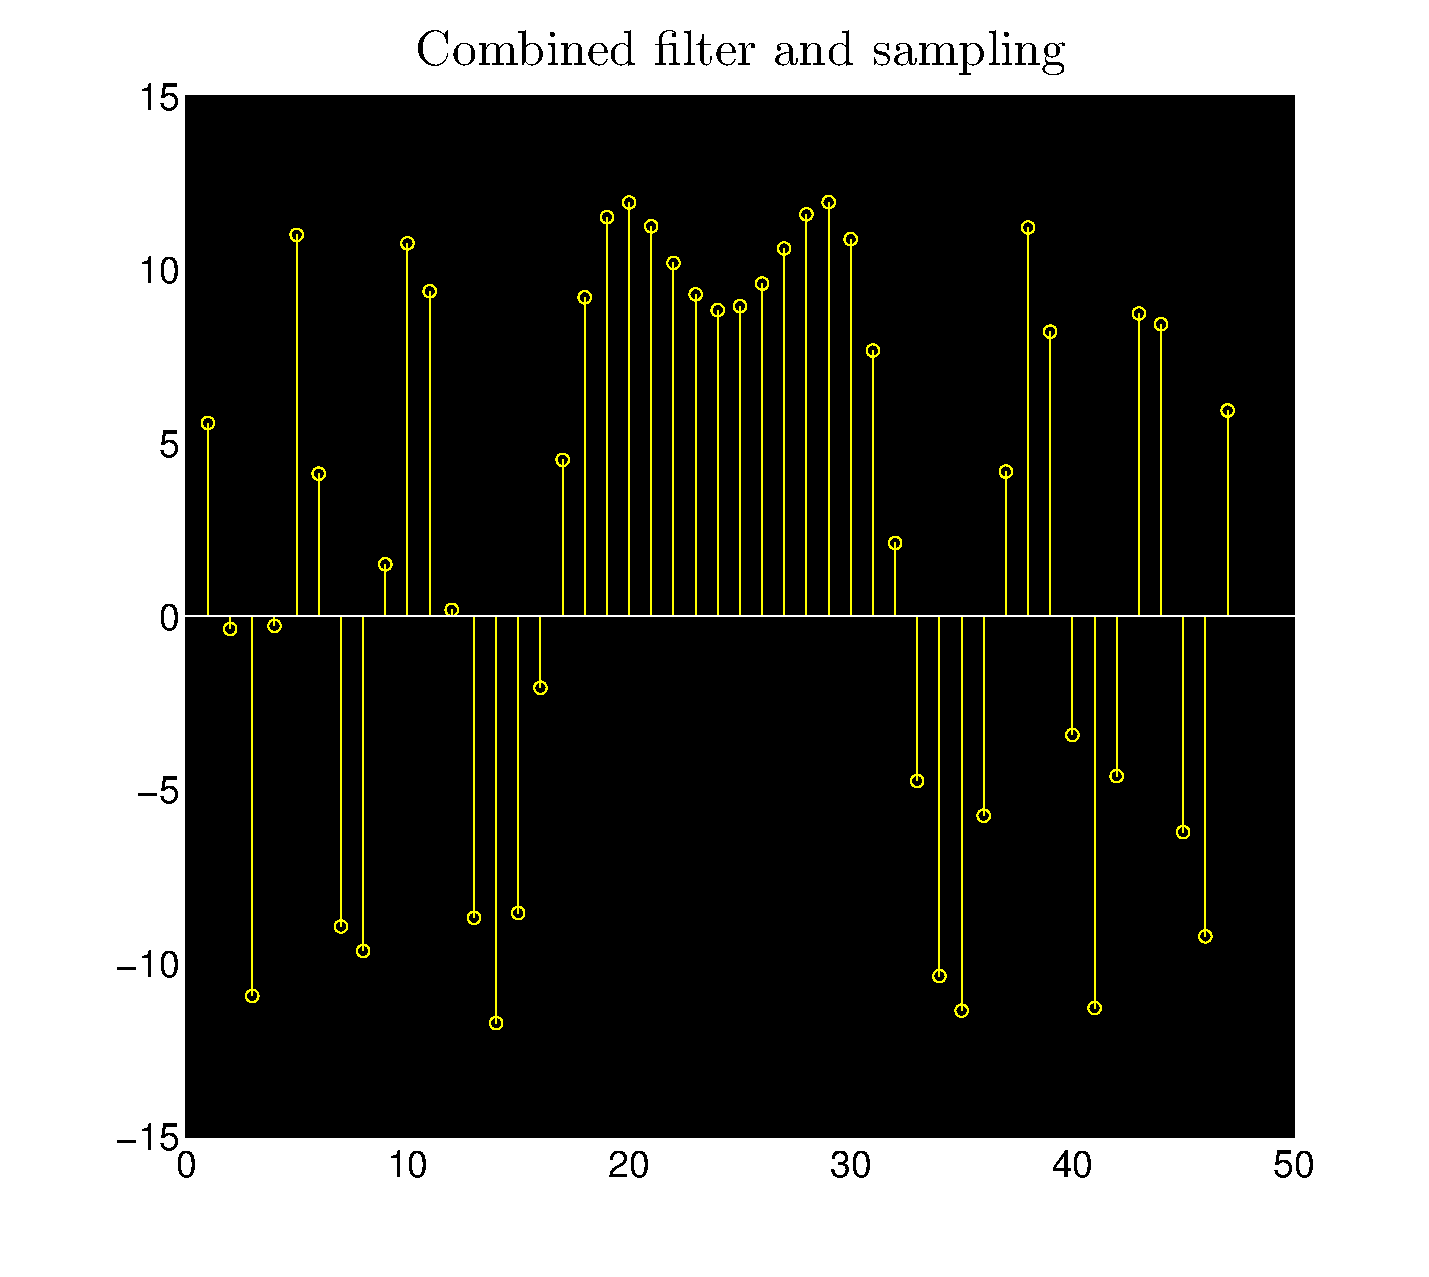
\includegraphics[width=1\textwidth]{Figures/SampledTxCombinedFilterSamp.pdf}
\end{figure}
        \end{column}
         \begin{column}{.5\textwidth}

   \begin{figure}
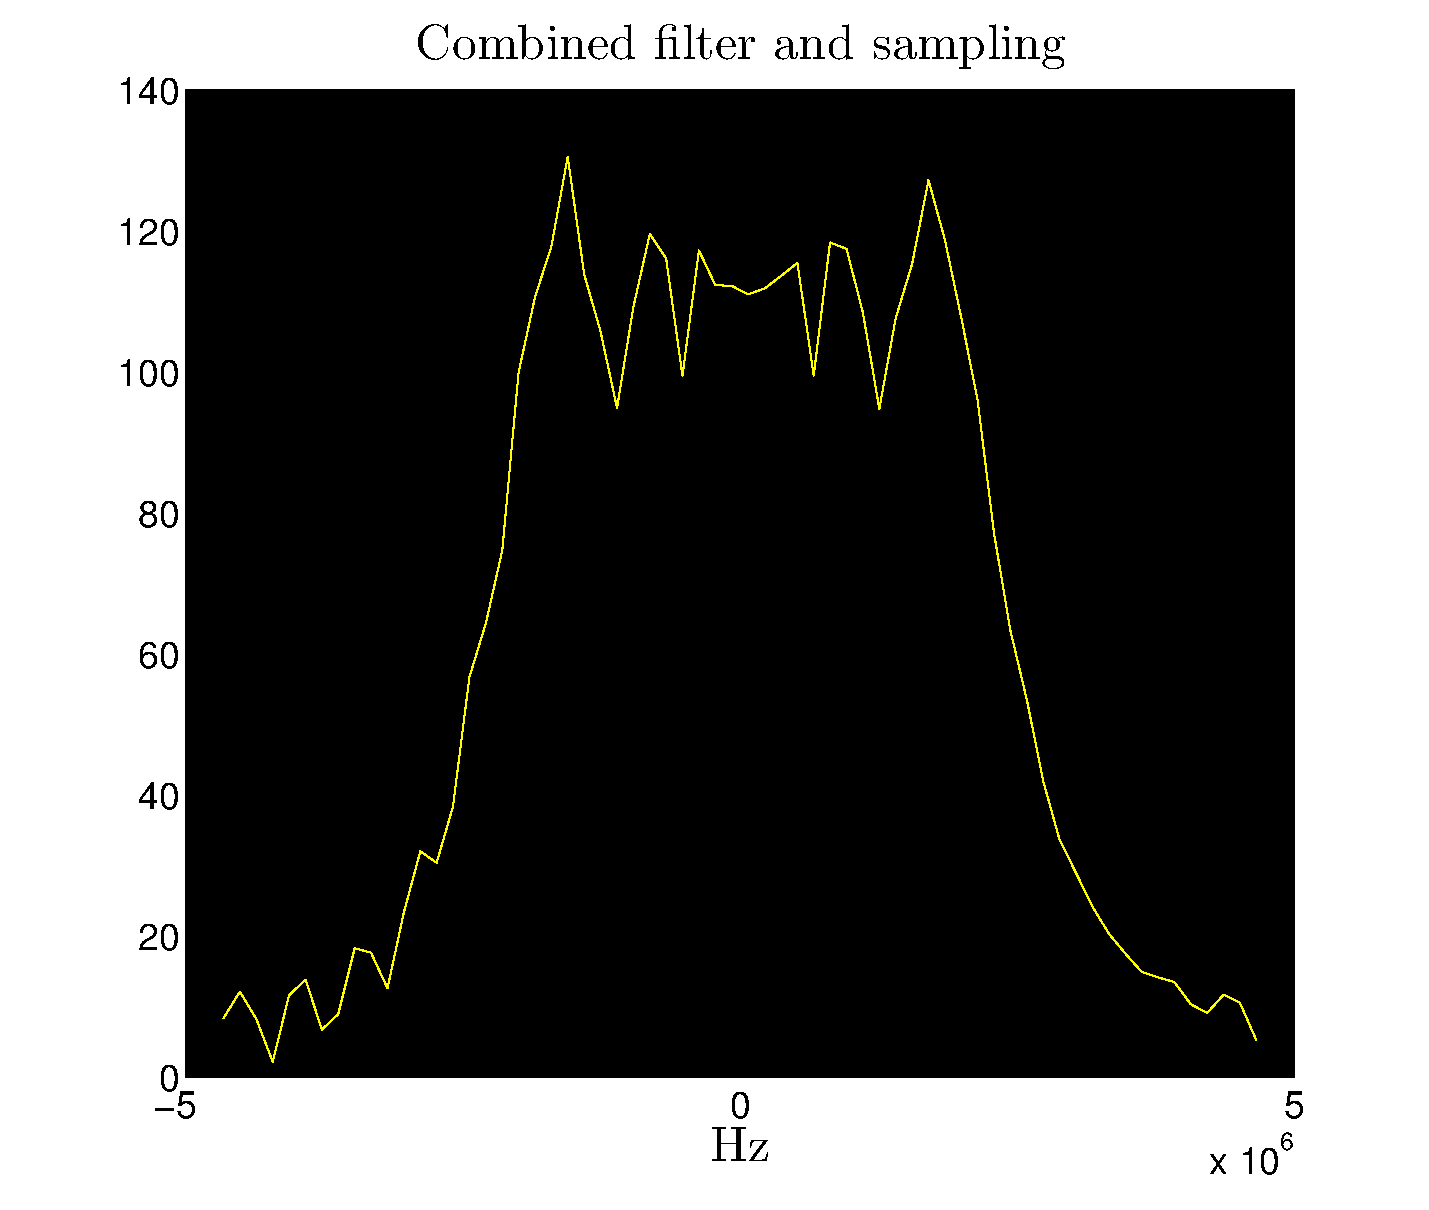
\includegraphics[width=1\textwidth]{Figures/SampledTxCombinedFilterSampFft.pdf}
\end{figure}
        \end{column}
\end{columns}
\end{frame}


\begin{frame}
 \frametitle{Rescaled}
\begin{figure}
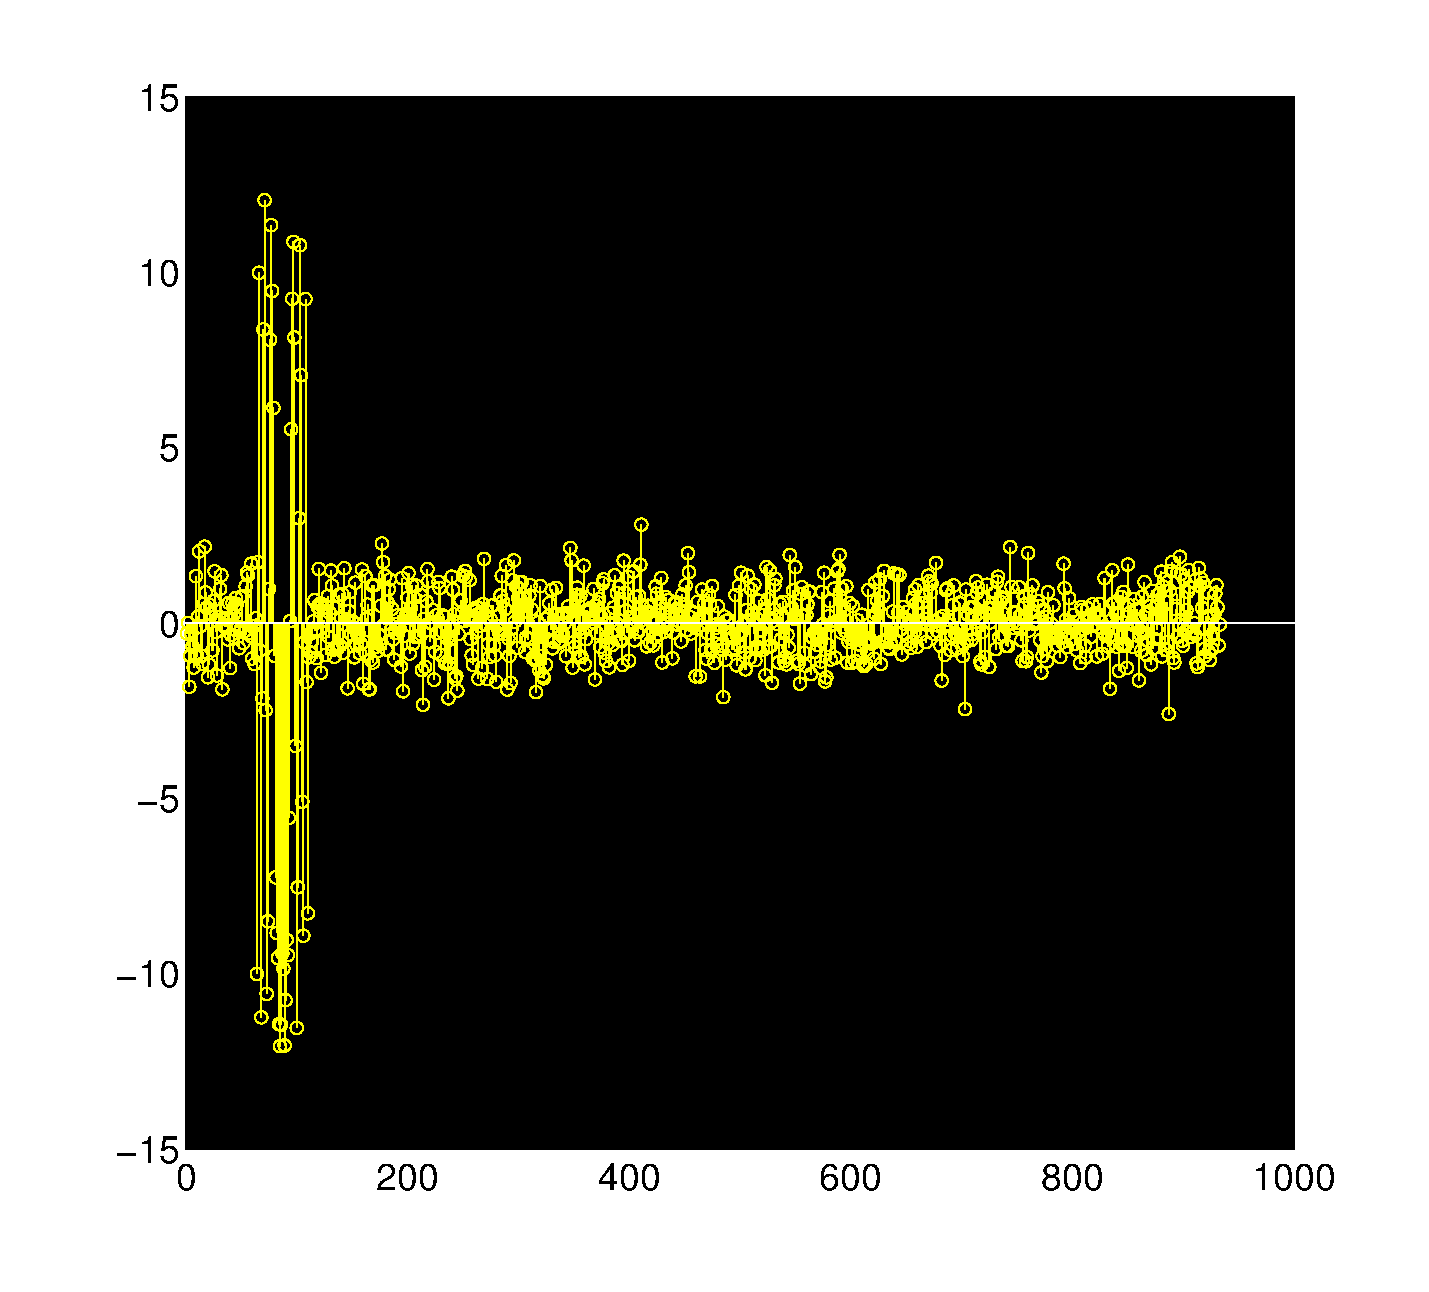
\includegraphics[width=0.75\textwidth]{Figures/SampledRxCombinedFilterSampRescale.pdf}
\end{figure}
\end{frame}

\begin{frame}
 \frametitle{Sampled  Rx}
\begin{figure}
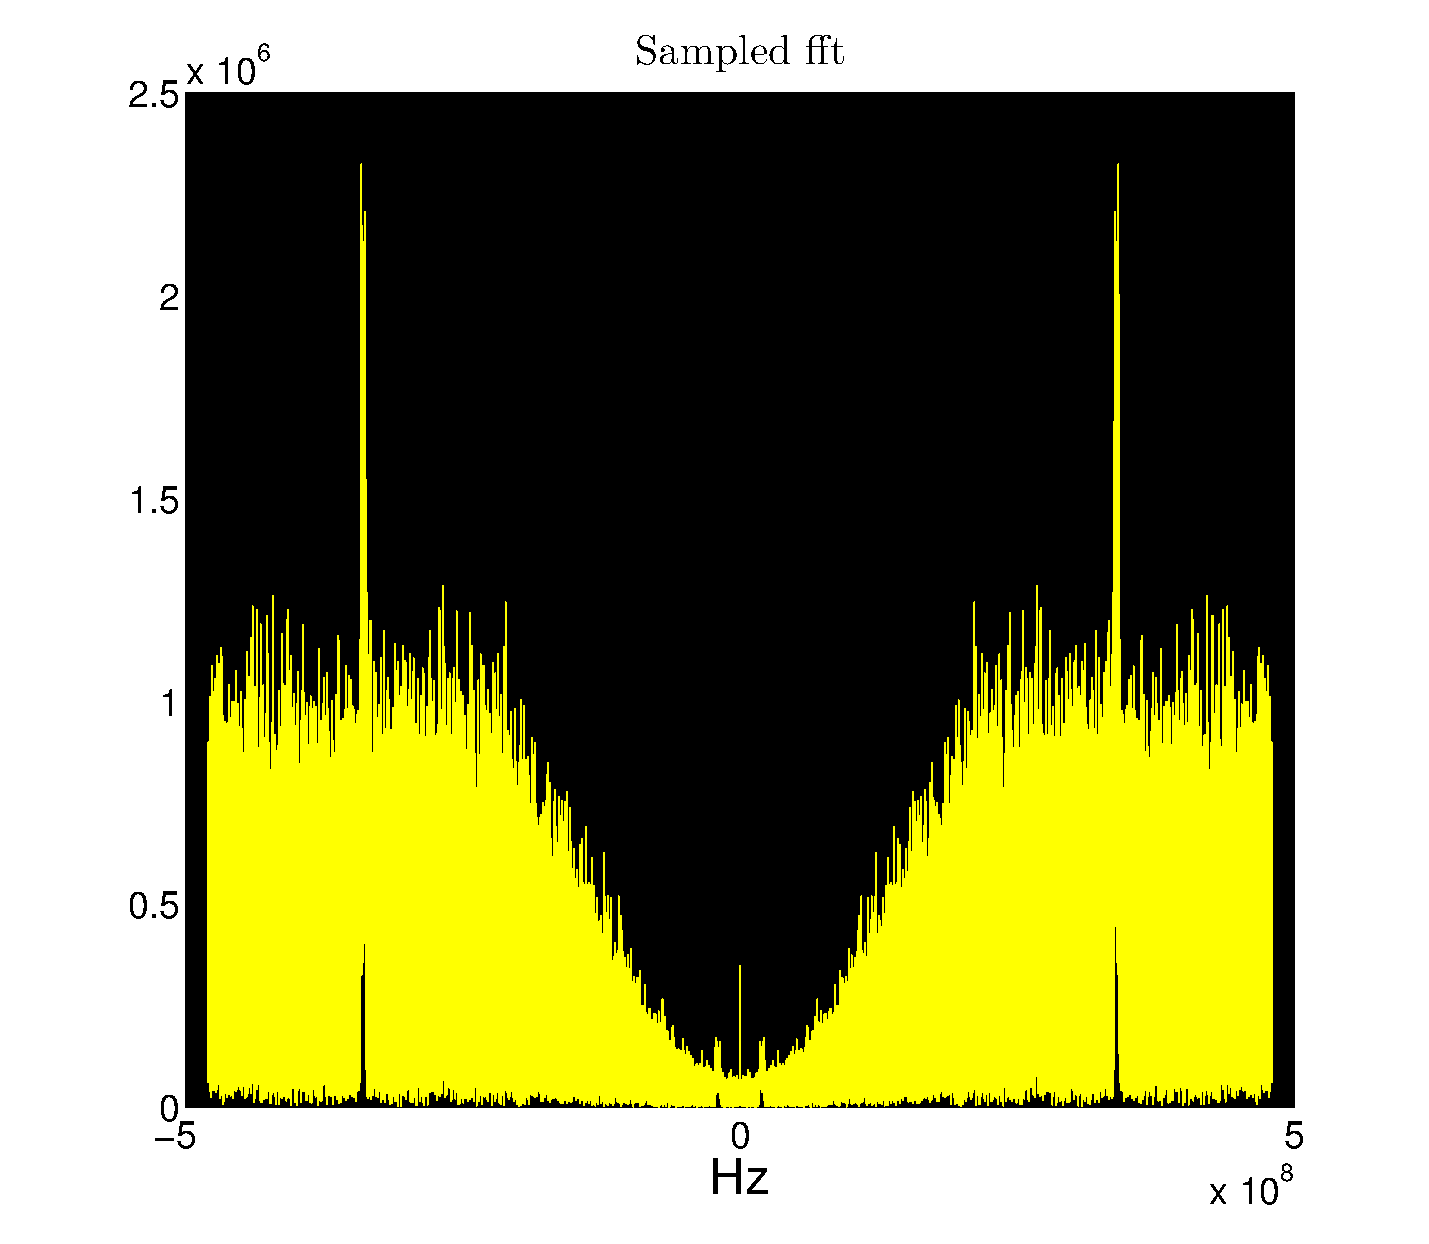
\includegraphics[width=0.75\textwidth]{Figures/SampledRxFft.pdf}
\end{figure}
\end{frame}

\begin{frame}
  \frametitle{Sampled  Rx high power input, cutoff}
\begin{figure}
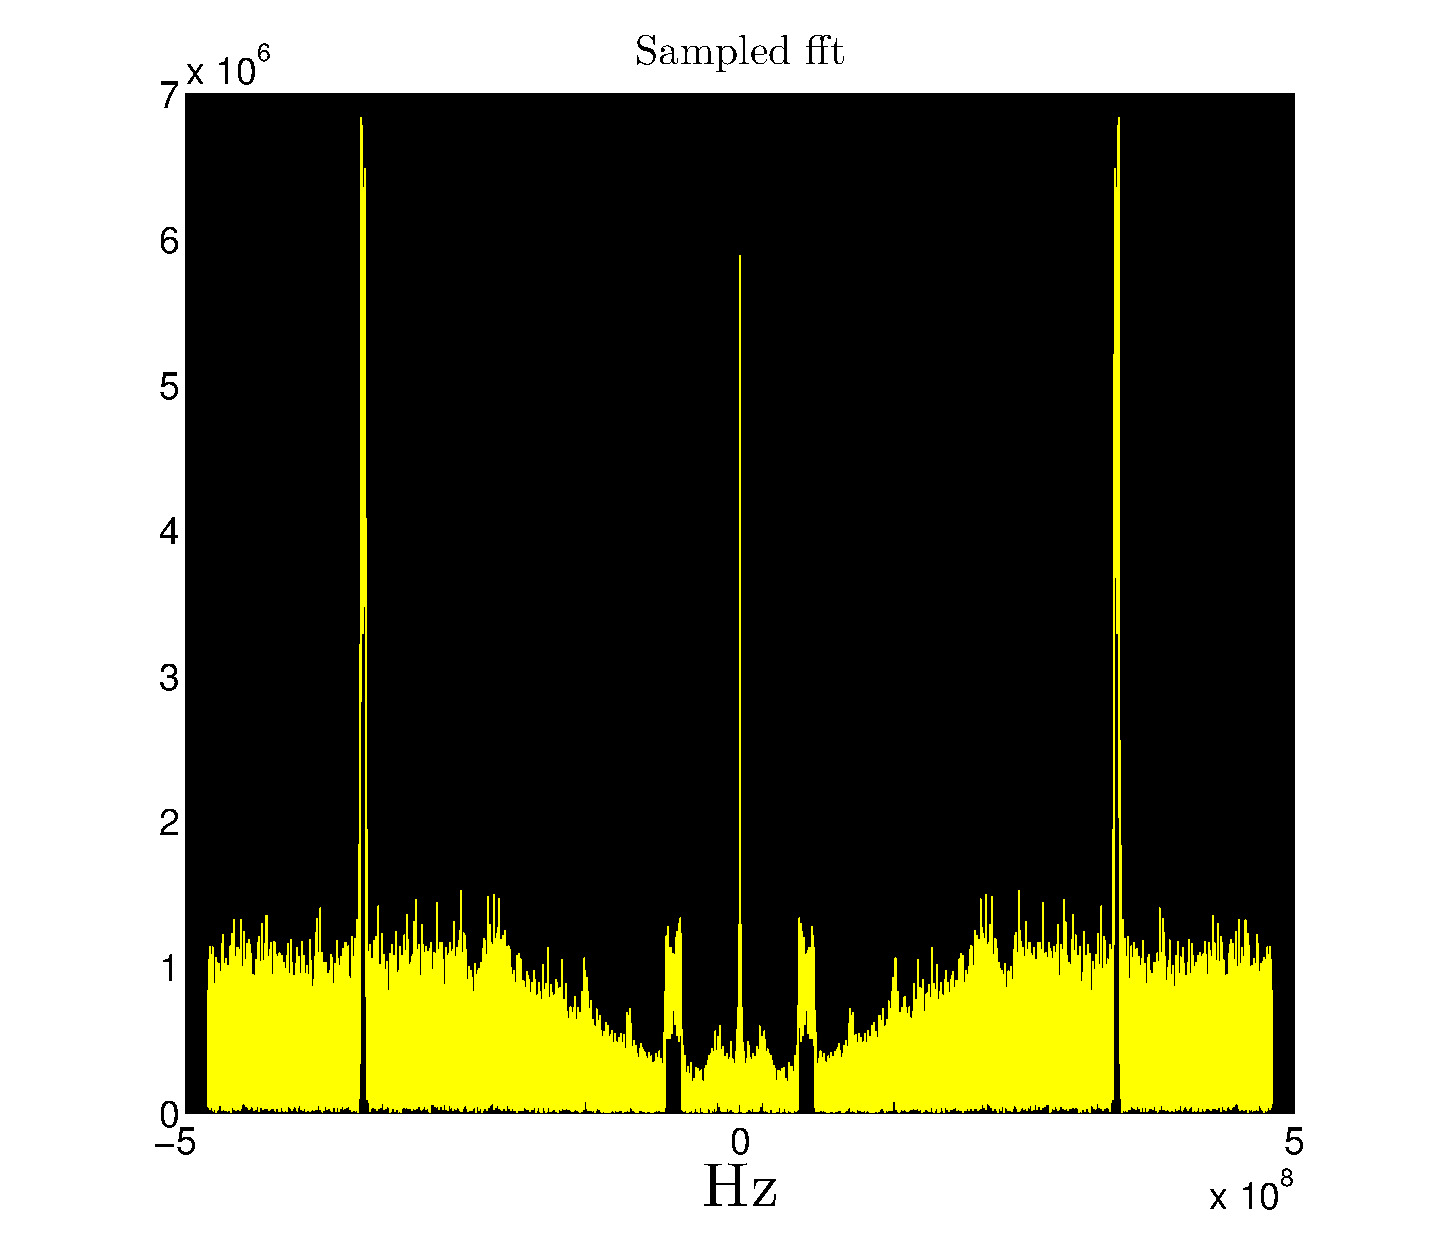
\includegraphics[width=0.75\textwidth]{Figures/SampledRxFftMattnad.pdf}
\end{figure}
\end{frame}






\begin{frame}
 \frametitle{Correlation of signal}
\framesubtitle{Abs}
 \begin{columns}[T]
        \begin{column}{.5\textwidth}
           
          \begin{figure}
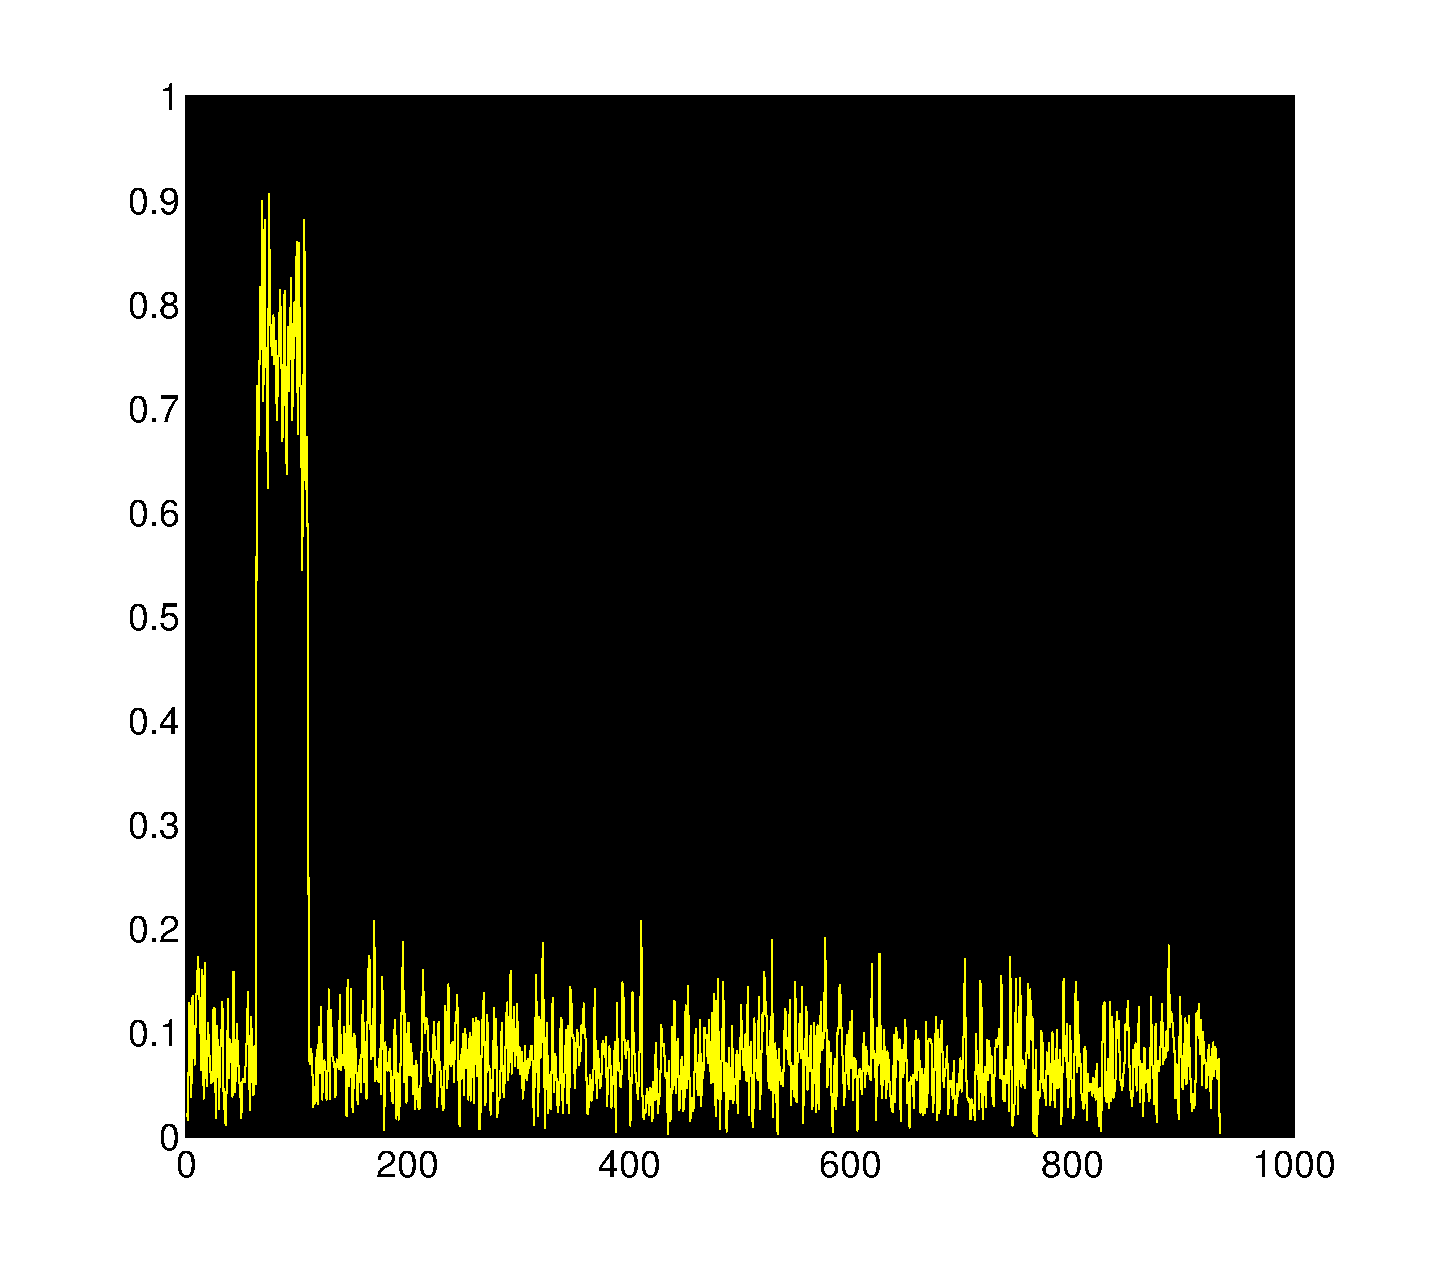
\includegraphics[width=1\textwidth]{Figures/SampledRx2DAbs.pdf}
\end{figure}
        \end{column}
         \begin{column}{.5\textwidth}

      \begin{figure}
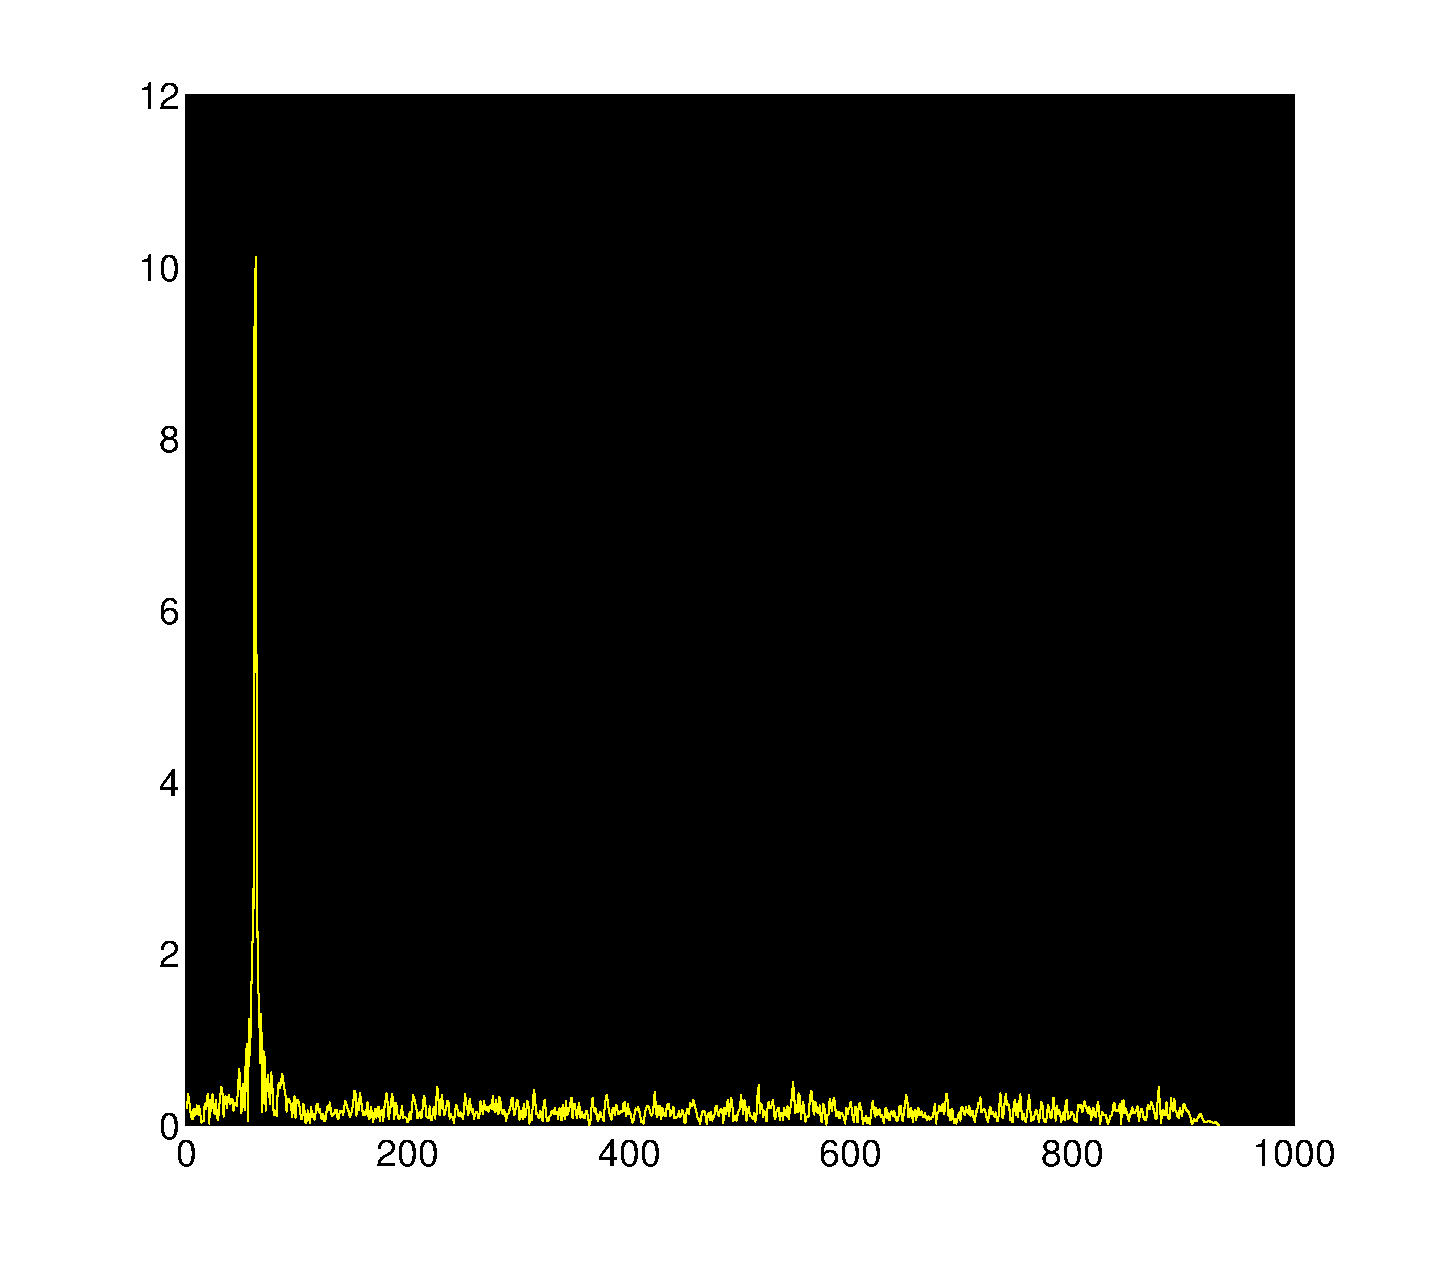
\includegraphics[width=1\textwidth]{Figures/SampledCorrelatedRx2DAbs.pdf}
\end{figure}
        \end{column}
\end{columns}
\end{frame}



\begin{frame}
 \frametitle{Correlation of signal}
\framesubtitle{Real}
 \begin{columns}[T]
        \begin{column}{.5\textwidth}
           
        \begin{figure}
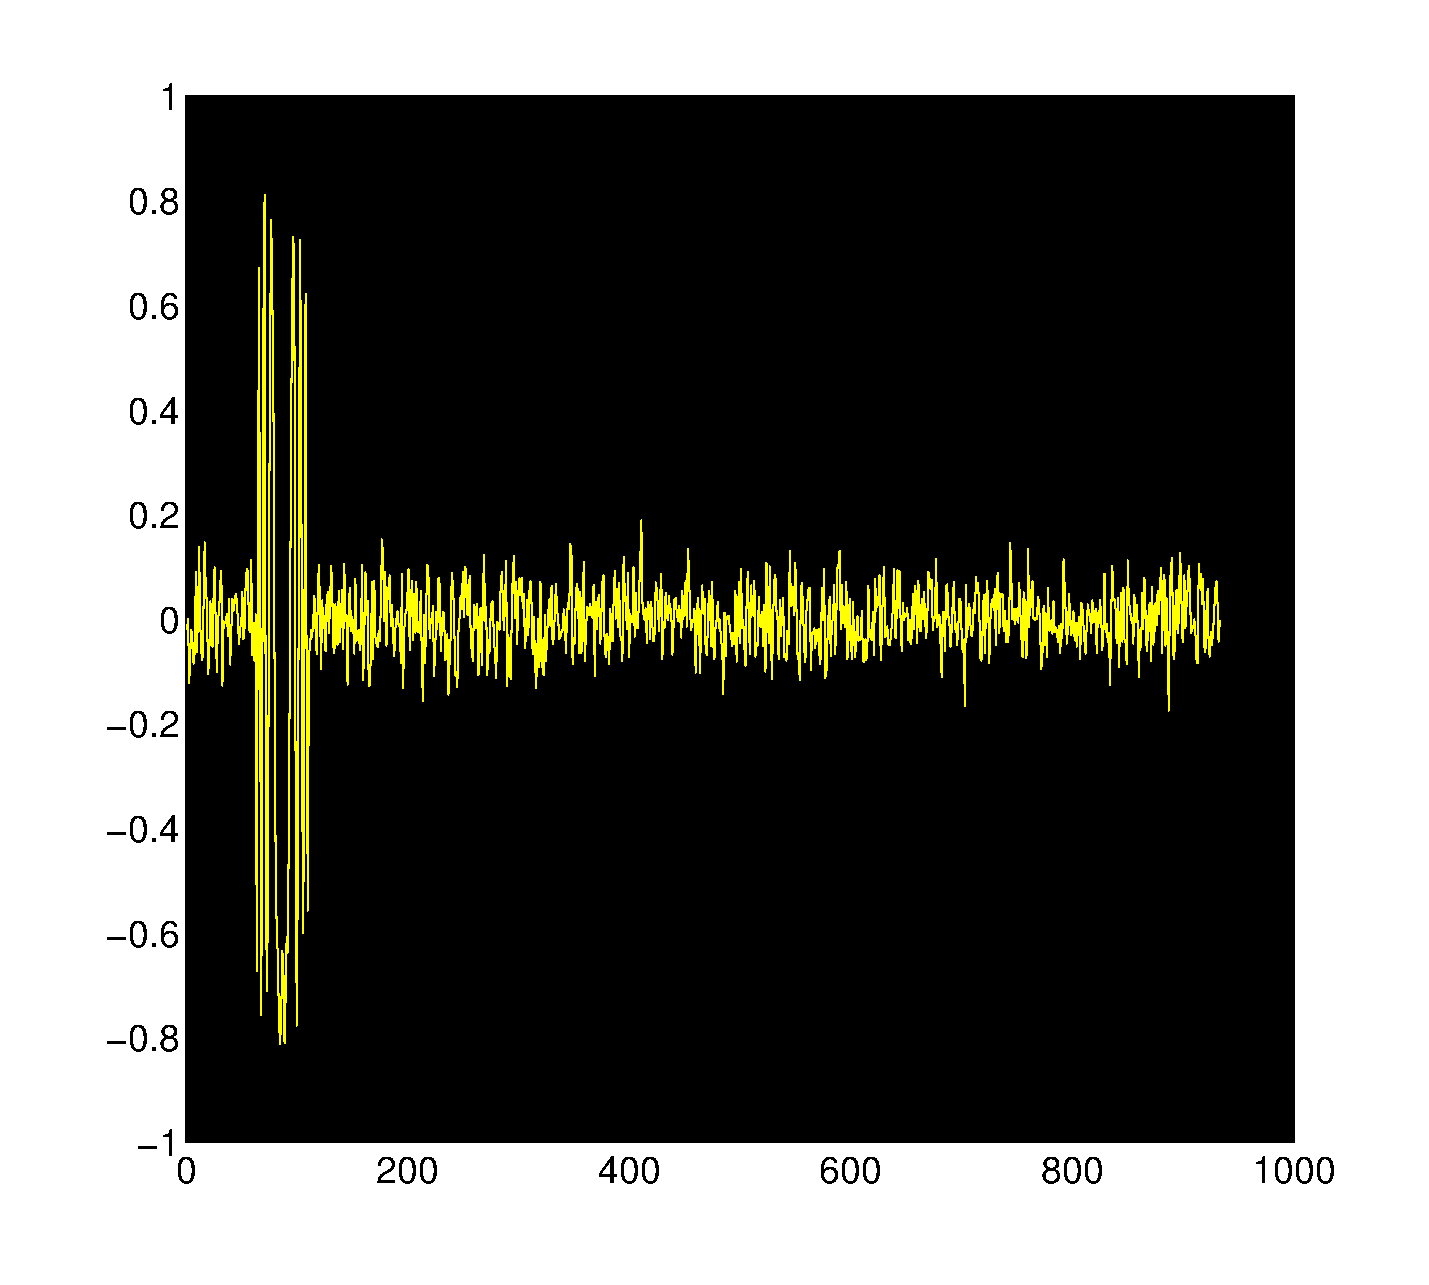
\includegraphics[width=1\textwidth]{Figures/SampledRx2DReal.pdf}
\end{figure}
        \end{column}
         \begin{column}{.5\textwidth}

     \begin{figure}
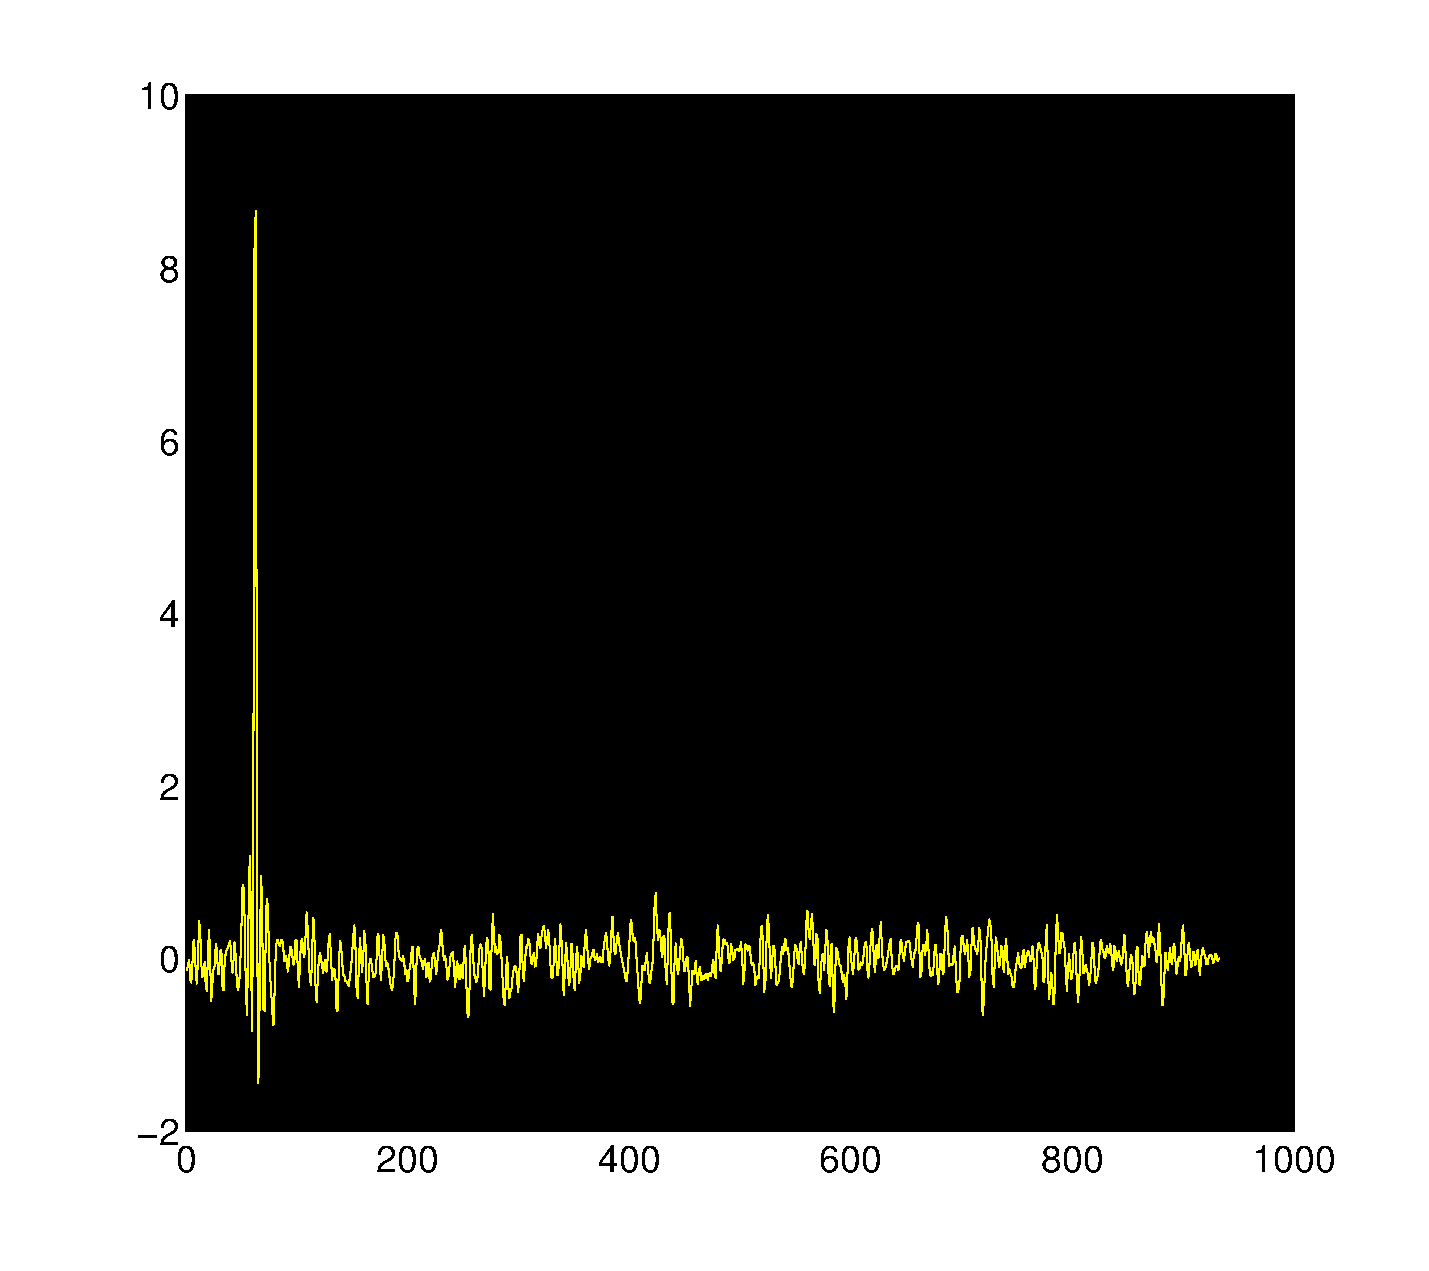
\includegraphics[width=1\textwidth]{Figures/SampledCorrelatedRx2DReal.pdf}
\end{figure}
        \end{column}
\end{columns}
\end{frame}




\begin{frame}
 \frametitle{Doppler plot}
\framesubtitle{$\sigma=1$m$^2$, 100m/s, 128 pulse}
\begin{figure}
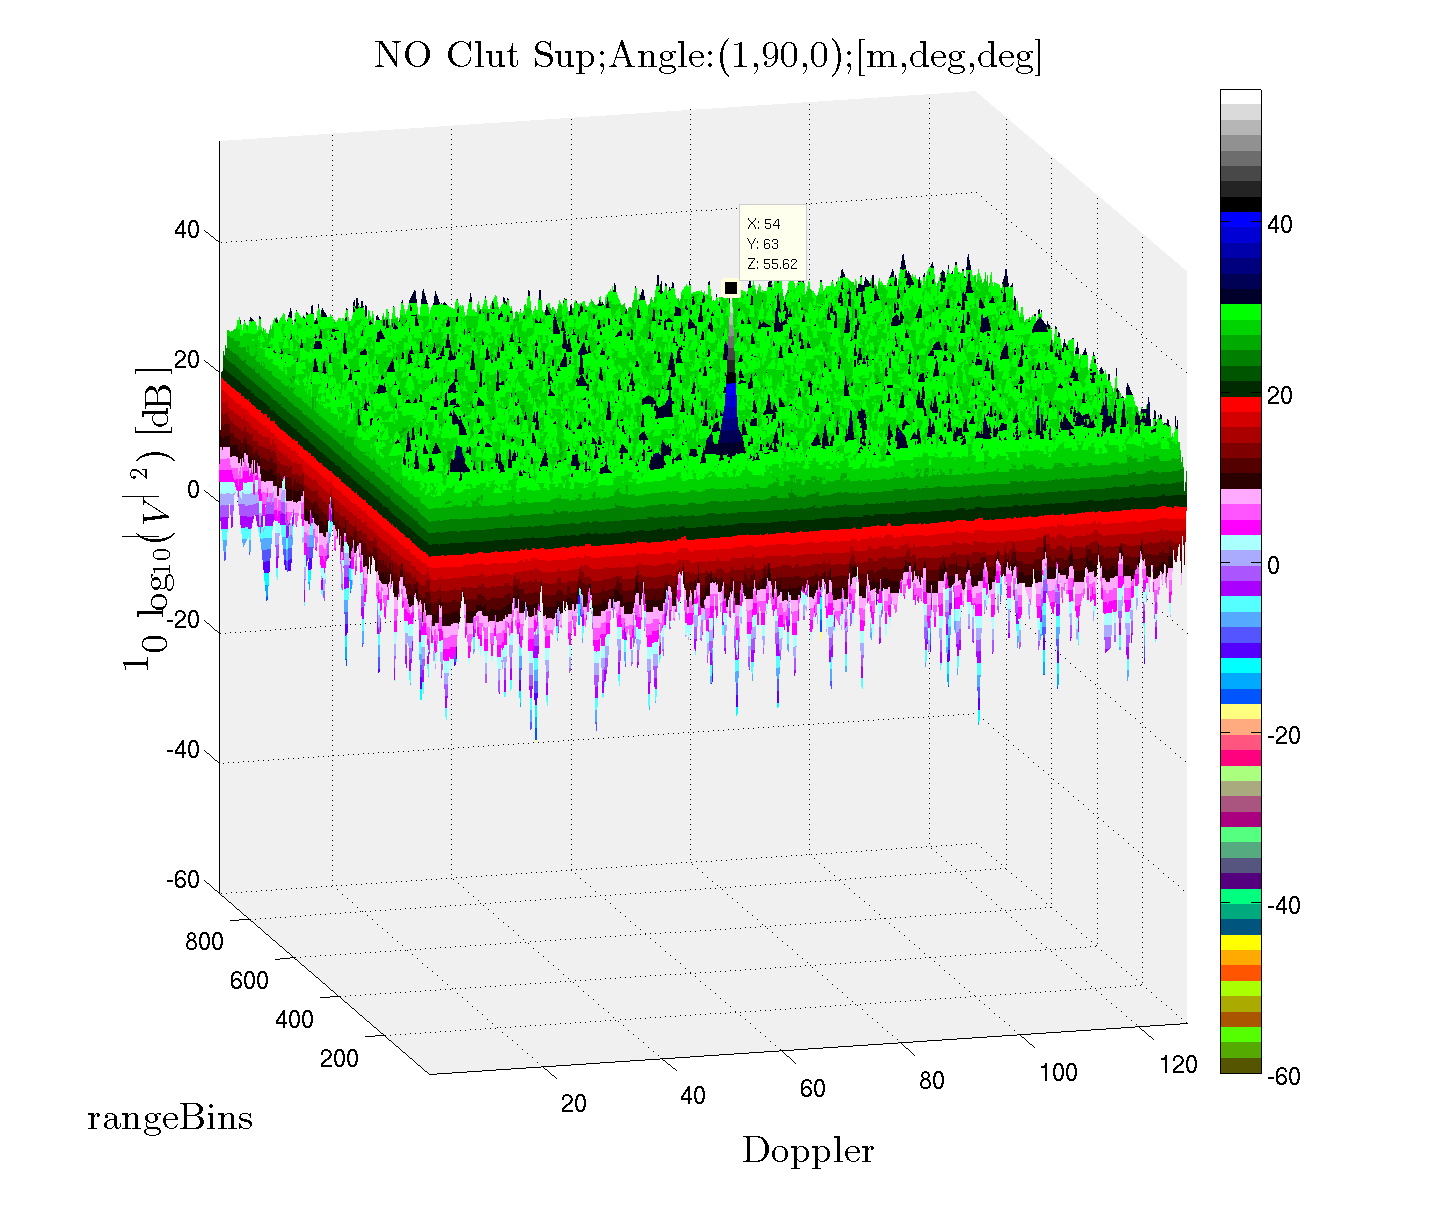
\includegraphics[width=0.8\textwidth]{Figures/DopplerSingleTarg1Km100ms128Puls.pdf}
\end{figure}
\end{frame}

\begin{frame}
\frametitle{Doppler plot}
\framesubtitle{$\sigma=1$m$^2$, 100m/s, 128 pulse and clutter echo from target with $\sigma=1e6$m$^2$}
   \begin{figure}
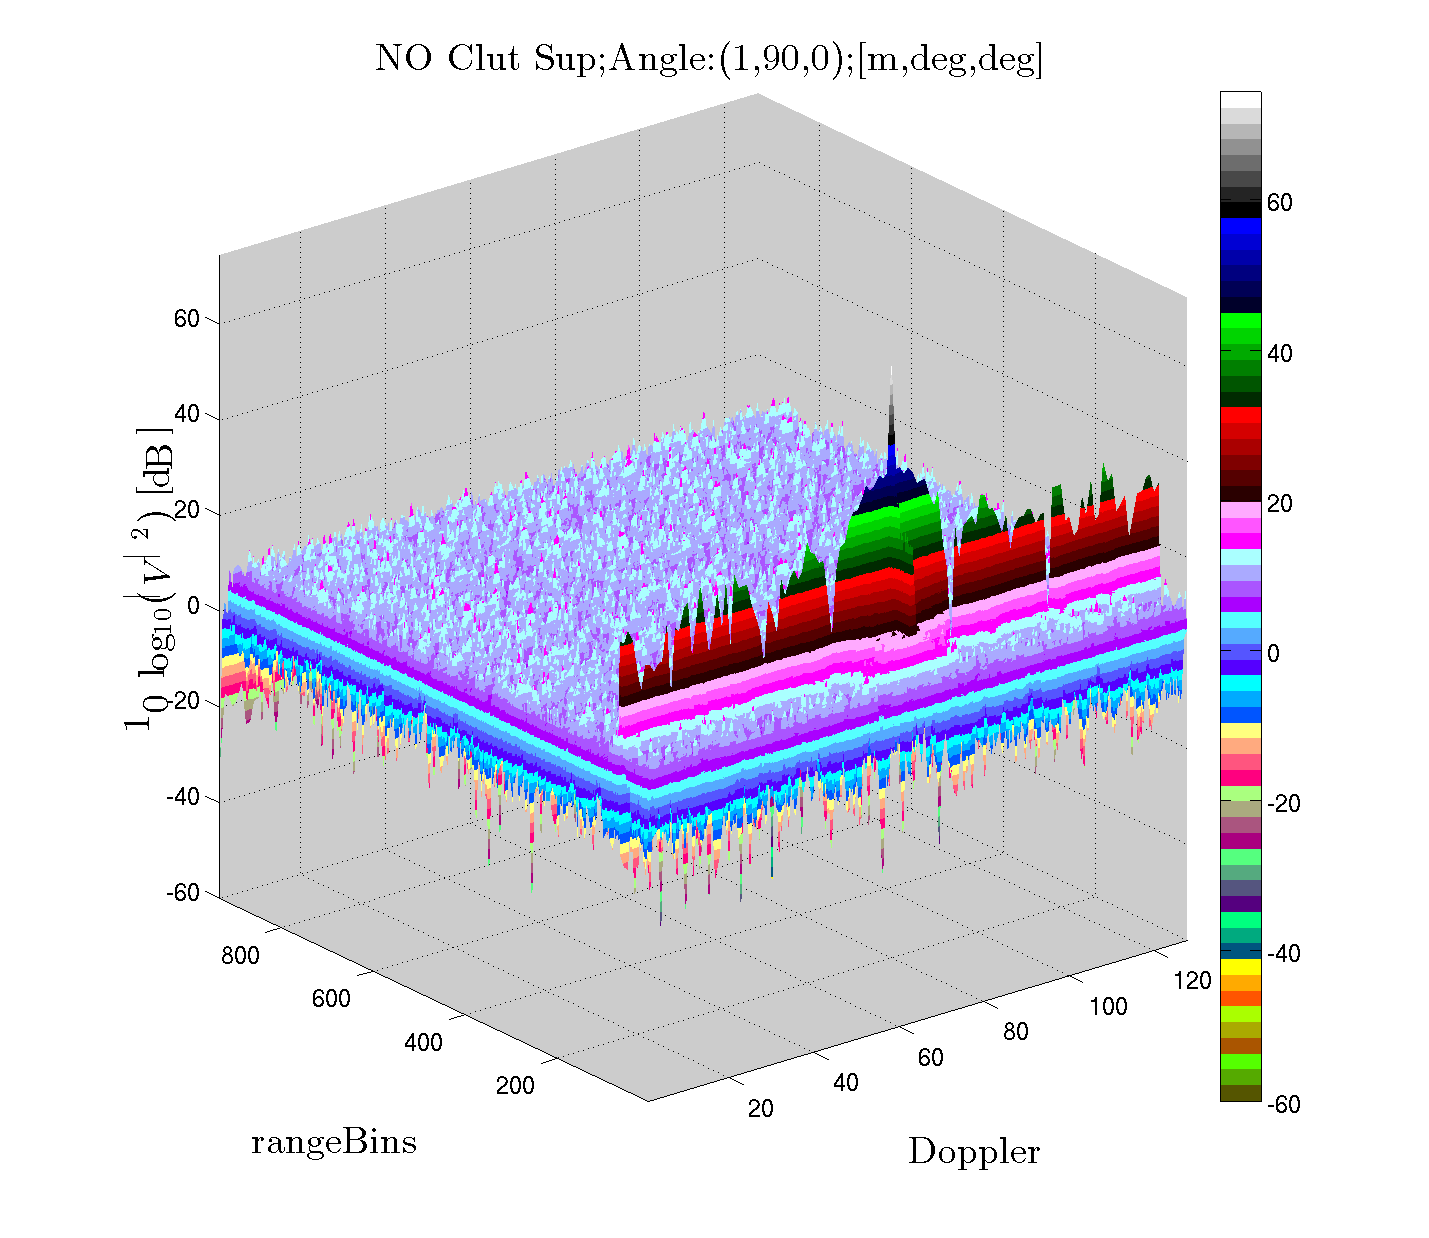
\includegraphics[width=0.8\textwidth]{Figures/Doppler1Km100ms128Puls.pdf}
\end{figure}
\end{frame}


\begin{frame}
 \frametitle{What's next?}
\begin{itemize}
\item Check least detectable input power 
\item Different scenarios


\end{itemize}

\end{frame}


\begin{frame}
 \frametitle{First title}
\begin{figure}
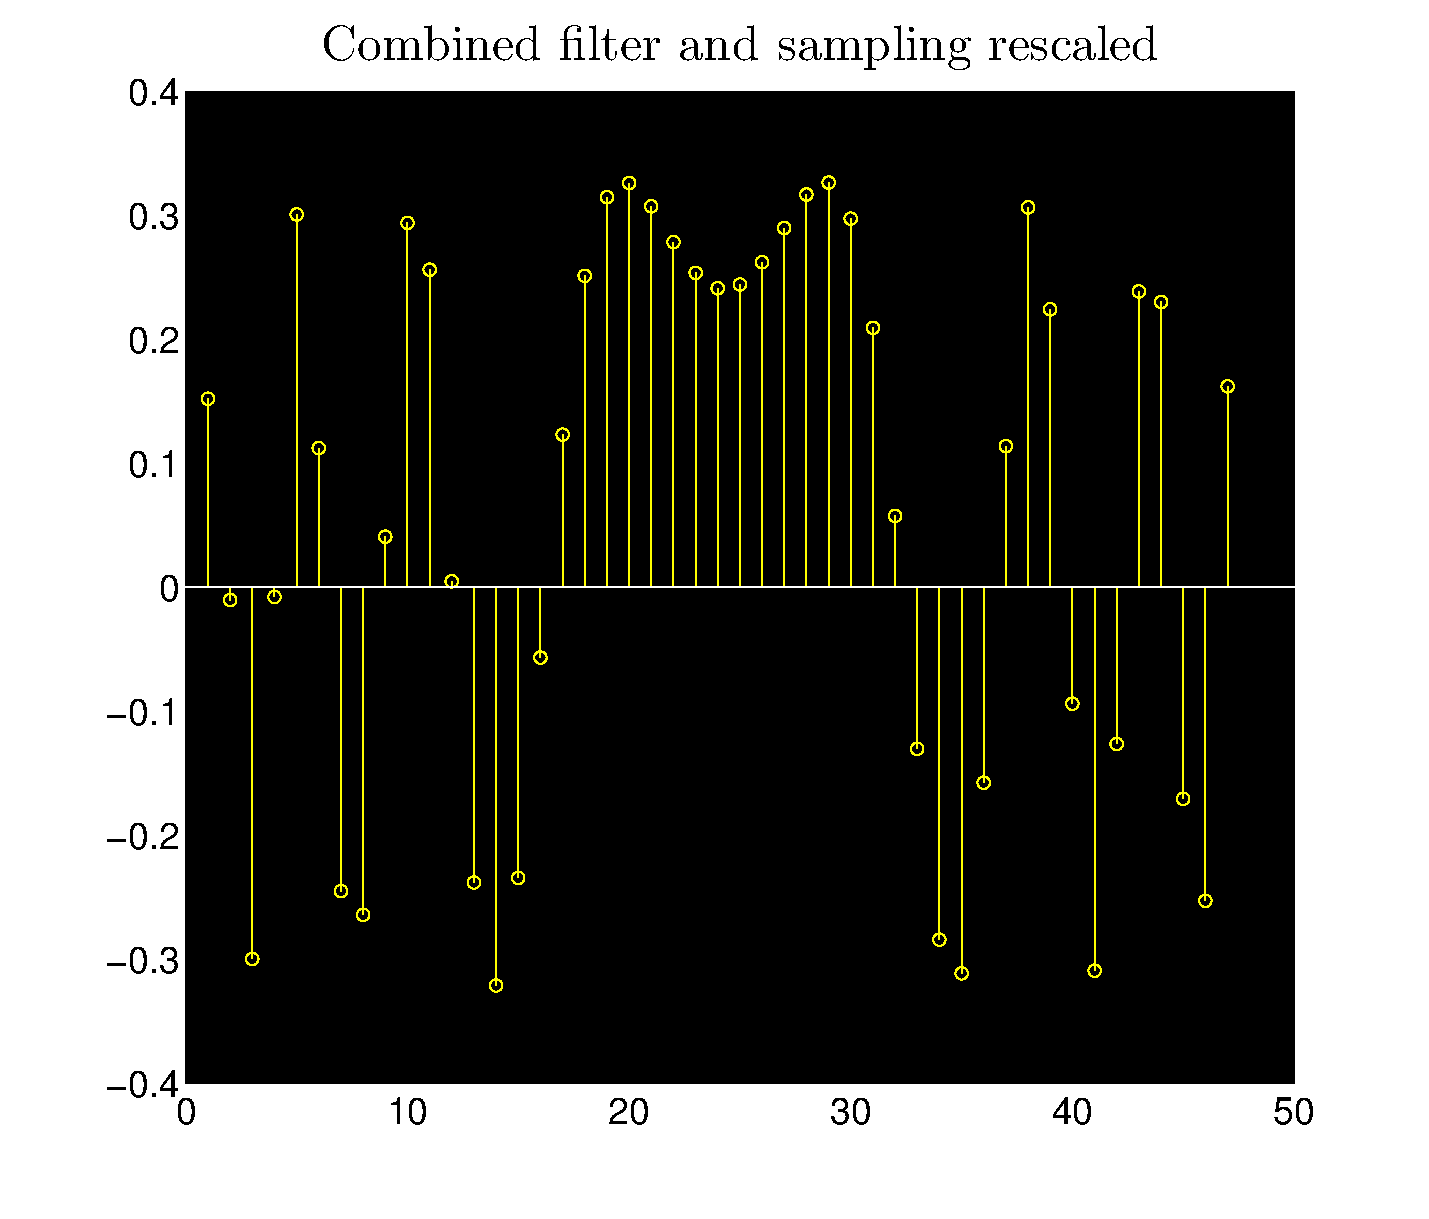
\includegraphics[width=0.75\textwidth]{Figures/SampledTxCombinedFilterSampRescale.pdf}
\end{figure}
\end{frame}



\begin{frame}
 \frametitle{First title}
\begin{figure}
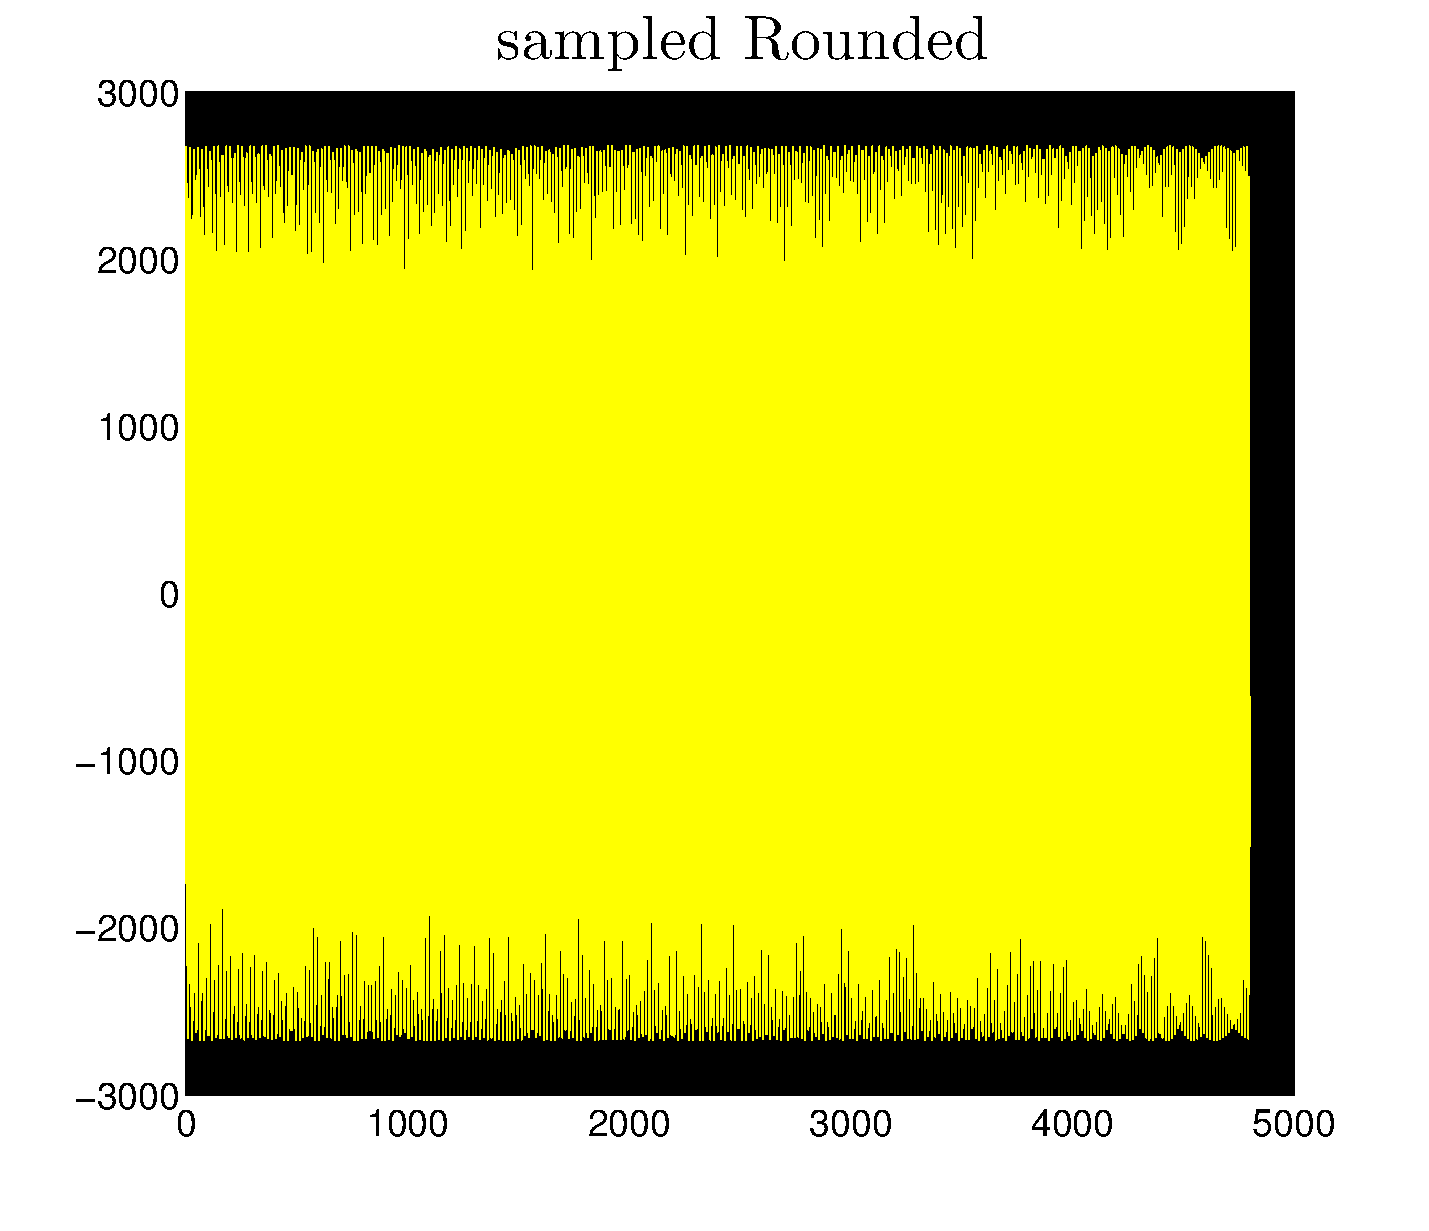
\includegraphics[width=0.75\textwidth]{Figures/SampledTxLevels.pdf}
\end{figure}
\end{frame}




\begin{frame}
 \frametitle{First title}
\begin{figure}
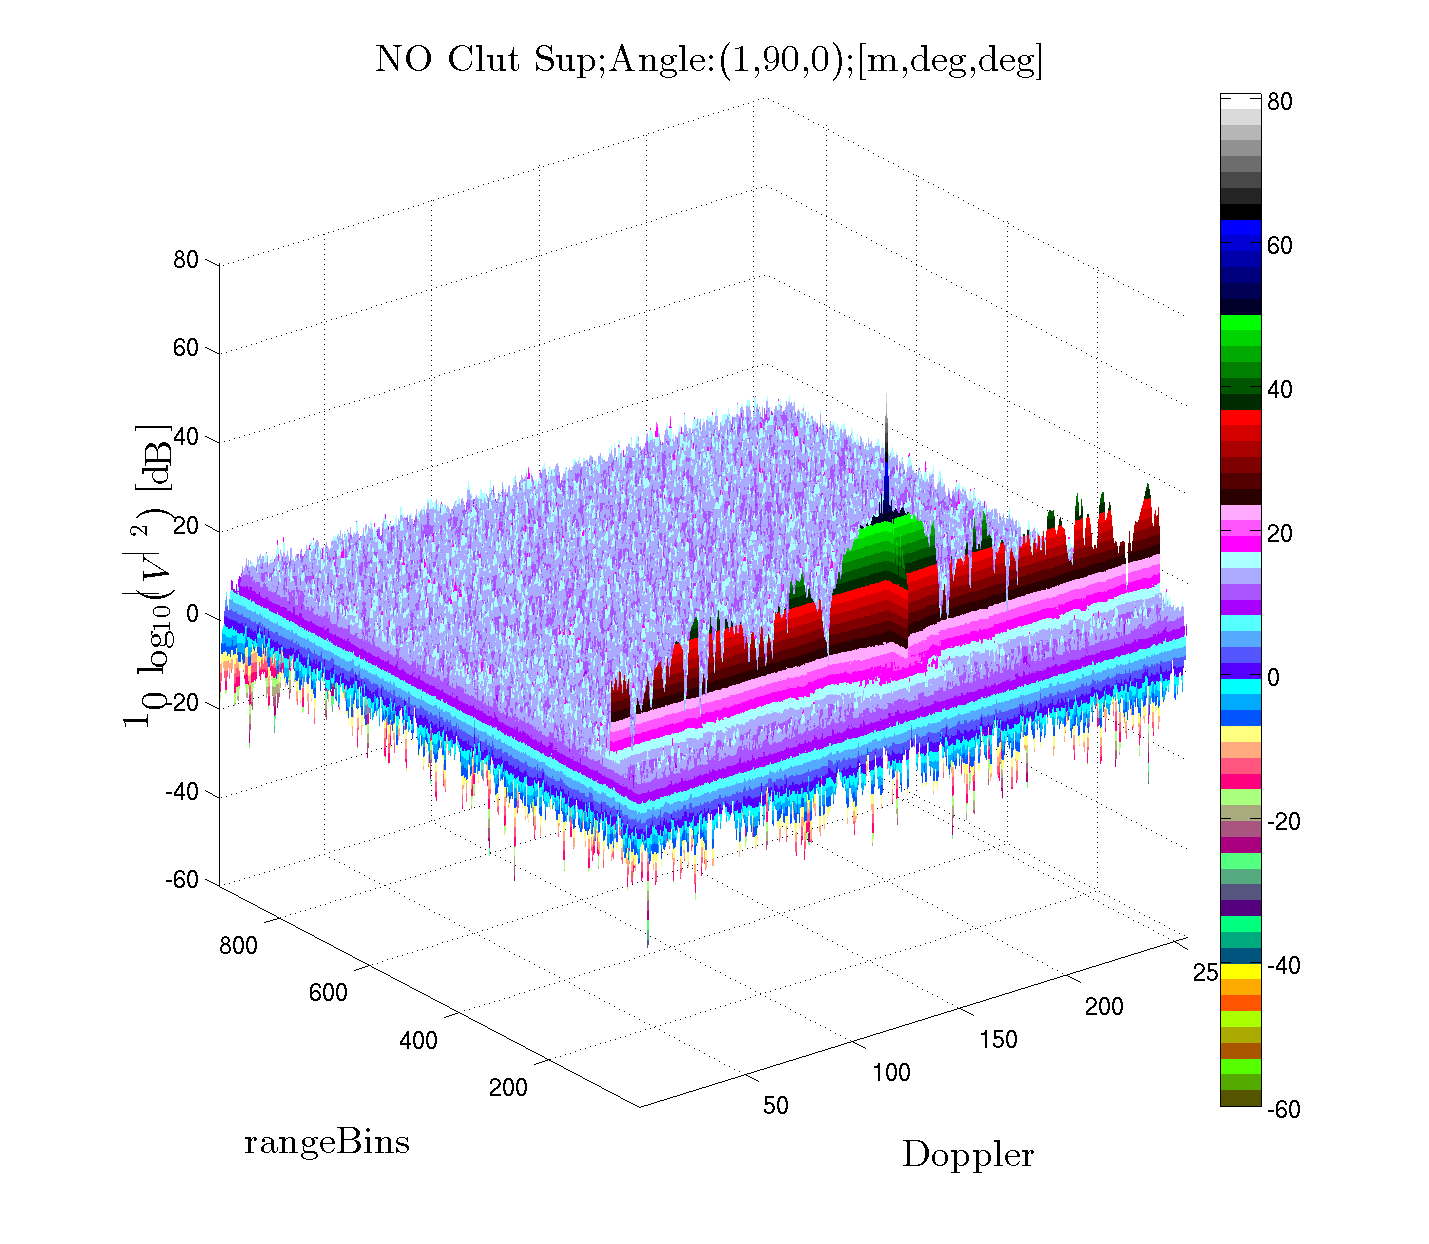
\includegraphics[width=0.75\textwidth]{Figures/Doppler1Km100ms256Puls.pdf}
\end{figure}
\end{frame}




\end{document}
